
%\documentclass[preprint,12pt]{elsarticle}

%% Use the option review to obtain double line spacing
%% \documentclass[authoryear,preprint,review,12pt]{elsarticle}

%% Use the options 1p,twocolumn; 3p; 3p,twocolumn; 5p; or 5p,twocolumn
%% for a journal layout:
 \documentclass[final,1p,times]{elsarticle}
%% \documentclass[final,1p,times,twocolumn]{elsarticle}
%% \documentclass[final,3p,times]{elsarticle}
%% \documentclass[final,3p,times,twocolumn]{elsarticle}
%% \documentclass[final,5p,times]{elsarticle}
%% \documentclass[final,5p,times,twocolumn]{elsarticle}

%% For including figures, graphicx.sty has been loaded in
%% elsarticle.cls. If you prefer to use the old commands
\usepackage{epsfig}

%% The amssymb package provides various useful mathematical symbols
\usepackage{amssymb}
%% The amsthm package provides extended theorem environments
\usepackage{amsthm}

\usepackage{amsmath}

\usepackage{CJK}
\usepackage{color}

\usepackage{enumitem}
\usepackage{rotating}

%% The lineno packages adds line numbers. Start line numbering with
%% \begin{linenumbers}, end it with \end{linenumbers}. Or switch it on
%% for the whole article with \linenumbers.
%% \usepackage{lineno}

%\journal{Nuclear Physics B}

\hyphenation{data-log}

\begin{document}

\newtheorem{theorem}{Theorem}
\newtheorem{definition}{Definition}
\newtheorem{example}{Example}
\newtheorem{lemma}{Lemma}
\newtheorem{corollary}{Corollary}

\begin{frontmatter}

%% Title, authors and addresses

%% use the tnoteref command within \title for footnotes;
%% use the tnotetext command for theassociated footnote;
%% use the fnref command within \author or \address for footnotes;
%% use the fntext command for theassociated footnote;
%% use the corref command within \author for corresponding author footnotes;
%% use the cortext command for theassociated footnote;
%% use the ead command for the email address,
%% and the form \ead[url] for the home page:
%% \title{Title\tnoteref{label1}}
%% \tnotetext[label1]{}
%% \author{Name\corref{cor1}\fnref{label2}}
%% \ead{email address}
%% \ead[url]{home page}
%% \fntext[label2]{}
%% \cortext[cor1]{}
%% \address{Address\fnref{label3}}
%% \fntext[label3]{}

\title{Parallel Tractability of Ontology\\
Materialization: Technique and Practice}

%% use optional labels to link authors explicitly to addresses:
%% \author[label1,label2]{}
%% \address[label1]{}
%% \address[label2]{}

\author[add1]{Zhangquan Zhou \corref{cor1}}
\ead{quanzz1129@gmail.com}
\cortext[cor1]{Corresponding author}

\author[add1]{Guilin Qi}
\ead{gqi@seu.edu.cn}

\author[add2]{Birte Glimm}
\ead{birte.glimm@uni-ulm.de}

\address[add1]{
    School of Computer Science, Southeast University, China
}

\address[add2]{
    Institution of Artificial Intelligence, University of Ulm
}


\begin{abstract}
Materialization is an important reasoning service for applications built
on the ontology languages, such as OWL. With a
rapid growth of semantic data, it is challenging to perform
materialization on large-scale ontologies efficiently.
Current work proposes parallel algorithms and employs computing
platforms of high-performance to make materialization sufficiently efficient and scalable in practice.
However, there do exist ontologies, for which
materialization cannot always be improved by parallelism (we use experiments to show this in Section~\ref{sec:evaluation}).
On the other hand, some well-known large-scale ontologies, such as YAGO, have been shown to have
good performance for parallel reasoning, but they are expressed in ontology languages
that are not parallelly tractable in theory, i.e., the efficiency of reasoning may not be improved
on a parallel implementation.
This motivates us to study the problem of \emph{parallel tractability} of ontology
materialization from a theoretical perspective.
That is, we aim to identify the ontologies for which materialization is
parallelly tractable, i.e., in NC complexity.
The results of the parallel tractability can be further used to optimize
materialization algorithms and to guide ontology engineers in creating parallelly tractable ontologies.

In this work, we focus on datalog rewritable ontology languages.
We propose some algorithms, called NC algorithms, to identify several classes of datalog rewritable
ontologies (called \emph{parallelly tractable classes})
such that materialization over them is parallelly tractable.
We then investigate the parallel tractability of materialization over
two datalog rewritable ontology languages DL-Lite and DHL (\emph{Description Horn Logic}).
We show that materialization over any ontology expressed in DL-Lite$_{core}$ or DL-Lite$_\mathcal{R}$ is parallelly tractable.
For DHL, there exist ontologies where materialization can hardly be parallelized.
We propose to restrict the usage of DHL such that the restricted ontologies are parallelly tractable.
We further extend the results to an extension of DHL that also allows \emph{complex role inclusion axioms}.
To verify the practical usability of the above results, we analyze real-world datasets and show
that many ontologies expressed in DHL or its extension belong to
the parallelly tractable classes. Based on the results of parallel tractability,
we further implement an optimized parallel algorithm
and compare it to the state-of-the-art reasoner RDFox. The experimental results show that the
optimization used in our implementation results in a better
performance on parallelly tractable ontologies compared with RDFox.
\end{abstract}

\begin{keyword}
ontology \sep materialization \sep datalog \sep parallel tractability \sep NC complexity
\end{keyword}

\end{frontmatter}

%% \linenumbers


\section{Introduction}
\label{sec:introduction}

The Web Ontology Language (OWL)\footnote{The latest version is OWL 2: http://www.w3.org/TR/owl2-overview/}
is an important standard for ontology language in the Semantic Web and knowledge-based applications.
In these applications, \emph{materialization}, which is the reasoning task of computing all implicit
facts that follow from a given ontology \cite{handbook}, plays an important role. By means of it, developers and users
can optimize query answering, ontology diagnosis and debugging. Since huge amounts of semantic data
are being generated at an increasing pace by sensor networks, government authorities and social
media \cite{LehmbergRMB16,MeuselBP15}, it is challenging to conduct materialization on such large-scale ontologies efficiently.

There has been work proposing parallel reasoning algorithms and employing parallel computing platforms
for the ontology language RDFS and its extended
fragments \cite{MotikNPHO14,PetersSZ15,SubercazeGCL16}. Several optimization strategies, e.g., dictionary encoding, balancing workload
and data partitioning, are further studied to enhance parallel RDFS reasoning. There are also parallel implementations for scalable
reasoning of highly expressive ontology languages \cite{SteigmillerLG14,WuH12}. On the other hand, several work utilizes different kinds of computing platforms to make reasoning tasks more efficient in parallel, such as supercomputers \cite{Hoeksema2011,GoodmanJMAAH11},
MapReduce \cite{UrbaniKMHB12} and GPU servers \cite{HeinoP12}.

The above work verifies the effectiveness of parallel reasoning based on the evaluations on different test datasets.
However, for most popular ontology languages, even RDFS and datalog rewritable ontology languages,
which have \texttt{PTime}-complete or higher complexity of reasoning in the worst case,
they are not parallelly tractable according to \cite{Raymond95}, i.e., the efficiency of reasoning may not be
improved on a parallel implementation. A possible reason of the high performance of parallel
reasoning is that the utilized test datasets do not fall in the worst cases in terms of computational complexity.
It has also been shown that some well-known large-scale ontologies, such as YAGO, have good performance for parallel
reasoning \cite{KolovskiWE10}, but they are expressed in ontology languages that are not parallelly tractable in theory.
On the other hand, there do exist ontologies for which materialization cannot
always be improved by parallelism (we use experiments to show this in Section~\ref{sec:evaluation}).
The current work of parallel ontology reasoning can hardly explain this.
While one can try out different parallel implementations to see whether an ontology can be handled by (one of) them efficiently,
we study the problem of parallel tractability in theory and identify properties that make an ontology parallelly tractable.
These properties can be further used to optimize parallel algorithms and to guide ontology engineers in creating ontologies
for which parallel tractability can be guaranteed theoretically.

According to \cite{MotikNPHO14}, many real large-scale ontologies are essentially expressed in the ontology languages
that can be rewritten into datalog rules. Thus, we focus on such datalog rewritable ontology languages in this paper.
The main target of this paper is to identify the classes of datalog rewritable ontologies such that materialization
over these ontologies is parallelly tractable, i.e., in the parallel complexity class NC \cite{Raymond95}.
This complexity class consists of problems that can be solved efficiently in parallel.
To show that a problem is in the NC class, one can give an \emph{NC algorithm} that handles this problem
in parallel computation \cite{Raymond95}.
An NC algorithm is required to terminate in parallel poly-logarithmic time.
However, current materialization algorithms of datalog rewritable ontology languages
(e.g., the core algorithm used in RDFox \cite{MotikNPHO14}) are not NC algorithms,
since they are designed for general datalog programs and has \texttt{PTime}-complete complexity.
Thus, we first give NC algorithms that perform materialization,
and then identify the corresponding classes of datalog rewritable ontologies (called \emph{parallelly tractable classes})
that can be handled by these NC algorithms. To make the proposed NC algorithms practical,
we also discuss how to optimize and implement them.

In the practical part of this work, we study specific datalog rewritable ontology languages.
We first focus on the ontology language DL-Lite to clarify how to apply the above NC algorithms
to study the parallel tractability of ontology materialization.
We show that DL-Lite$_{core}$ and DL-Lite$_\mathcal{R}$ are parallelly tractable.
We then study the ontology language Description Horn Logic (DHL) \cite{GrosofHVD03}, which is the intersection of datalog and OWL
in terms of expressivity. We give a case of a DHL ontology where materialization can hardly be parallelized.
Based on the analysis of this case, we propose to restrict the usage of DHL such that materialization over the
restricted ontologies can be handled by the proposed NC algorithms.
We further extend the results to an extension of DHL that also allows complex role inclusion axioms.
Finally, we analyze well-known benchmarks and real-world datasets and show that many real ontologies following the
proposed restrictions belong to the parallelly tractable classes.
We implement a system based on an optimized NC algorithm for DHL materialization.
We compare our system to the state-of-the-art reasoner RDFox.
The experimental results show that the optimization proposed in this paper results in a better performance on parallelly
tractable ontologies compared with RDFox.

The rest of the paper is organized as follows. In Section~\ref{sec:background}, we introduce some basic notions.
We then give two NC algorithms for ontology materialization in Section~\ref{sec:ptclass}.
We study the parallelly tractable materialization of DL-Lite, DHL and an extension of DHL in Section~\ref{sec:ptonto} respectively.
In Section~\ref{sec:practicalAlg},
we discuss how to optimize and implement the given NC algorithms.
We analyze real-world datasets and evaluate our implementation in Section~\ref{sec:evaluation}.
We then discuss related work in Section~\ref{sec:related} and conclude in Section~\ref{sec:conclusion}.
The detailed proofs of the theorems and the lemmas in this paper are given in the appendix.


\section{Background Knowledge}
\label{sec:background}

In this section, we introduce some basic notions that are needed to introduce our approach.


\subsection{Datalog}

We discuss the main issues in this paper using standard datalog notions.
In datalog \cite{database}, a \emph{term} is a variable or a constant. An \emph{atom} $A$
is defined by $A\equiv p(t_1,...,t_n)$ where $p$ is a \emph{predicate} (or \emph{relational})
name, $t_1,...,t_n$ are terms, and $n$ is the arity of $p$. If all the terms in an atom $A$ are
constants, then $A$ is called a \emph{ground atom}.
A datalog \emph{rule} is of the form: `$B_1,...,B_n\rightarrow H$',\footnote{In datalog rules, a comma
represents a Boolean conjunction `$\wedge$'.} where $H$ is referred to as
the \emph{head atom} and $B_1,...,B_n$ the \emph{body atoms}. Each variable in the head atom
of a rule must occur in at least one body atom of the same rule. A \emph{fact} is a rule of
the form `$\rightarrow H$', i.e., a rule with an empty body and the head $H$ being a ground atom.
A datalog program $P$ consists of rules and facts.
A \emph{substitution} $\theta$ is a partial mapping of variables to constants.
For an atom $A$, $A\theta$ is the result of replacing each variable $x$ in $A$
with $\theta(x)$ if the latter is defined. We call $\theta$ a \emph{ground substitution}
if each defined $A\theta$ is a ground atom.
A \emph{ground instantiation} of a rule is obtained by applying a ground substitution on all
the terms in this rule with respect to a finite set of constants occurring in $P$.
Furthermore the ground instantiation of $P$, denoted by $P^*$,
consists of all ground instantiations of rules in $P$.
The predicates occurring only in the body  of some rules are called \emph{EDB predicates},
while the predicates that may occur as head atoms are called \emph{IDB predicates}.


\subsection{DHL and DL-Lite}

In what follows, we use $\textbf{CN}$, $\textbf{RN}$ and $\textbf{IN}$
to denote three disjoint countably
infinite sets of \emph{concept names, role names}, and \emph{individual names} respectively.
The set of roles is defined as $\textbf{R}:=\textbf{RN}\cup\{R^-|R\in\textbf{RN}\}$
where $R^-$ is the \emph{inverse role} of $R$.
For ease of discussion, we focus on the \emph{simple forms} of axioms shown
in the left column of Table~1. These simple forms can be obtained by using
well-known \emph{structure transformation} techniques \cite{KrotzschRH07,Kazakov09}.

DHL (short for \emph{description horn logic}) \cite{GrosofHVD03} is introduced as an
intersection of description logic (DL) and datalog in terms of expressivity.
We define a DHL ontology $\mathcal{O}$ as a triple:
$\mathcal{O}=\langle\mathcal{T},\mathcal{R},\mathcal{A}\rangle$, where
$\mathcal{T}$ denotes the TBox containing axioms of the forms (T1-T3);
$\mathcal{R}$ is the RBox that is a set of axioms of the forms (R1-R3);
$\mathcal{A}$ is the ABox containing \emph{assertions} of the forms (A1) and (A2).
In an axiom of either of  the forms (T1-T3 and R1-R3), concepts $A_{(i)}$ and $B$ are either
concept names, \emph{top concept} ($\top$) or \emph{bottom concept} ($\bot$); $R$ and $S_{(i)}$
are roles in $\textbf{R}$.
For an axiom of the form $A\sqsubseteq\forall R.B$ that is also allowed in DHL, we only consider its
equivalent form $\exists R^-.A\sqsubseteq B$.

DHL is related with other ontology languages.
First, DHL is essentially a fragment of the description logic Horn-$\mathcal{SHOIQ}$ with
disallowing \emph{nominal}, \emph{number restriction} and
right-hand \emph{existential restriction} ($A\sqsubseteq\exists R.B$).
Second, the expressivity of DHL covers that of RDFS to some extent \cite{GrosofHVD03}.
Reasoning with RDFS ontologies is \texttt{NP}-complete \cite{Horst05}
and, thus, is not parallelly tractable.
However, by applying some simplifications and restrictions, RDFS ontologies can be
expressed in DHL \cite{GrosofHVD03} that has \texttt{PTime}-complete complexity for
materialization.

\begin{table}
\begin{center}
\begin{tabular}{lcc}
\multicolumn{3}{c}{\textbf{Table 1: Axioms and corresponding datalog rules}}\\
\hline
&~~~~~~~~~~~~~~~~~~~~~~~~Axioms~~~~~~~~~~~~~~~~~~~~~~~~&~~~~~~~~~~~~~~~~~~~~~~~~Datalog Rules~~~~~~~~~~~~~~~~~~~~~~~~\\
\hline
\hline
(T1)& $A\sqsubseteq B$& $A(x)\rightarrow B(x)$\\
(T2)& $A_1\sqcap A_2\sqsubseteq B$& $A_1(x), A_2(x)\rightarrow B(x)$\\
(T3)& $\exists R.A\sqsubseteq B$& $R(x,y), A(y)\rightarrow B(x)$\\
(T4)& $A\sqsubseteq\exists R$& $A(x)\rightarrow R(x, o_{R}^A)$\\

\hline
(R1)& $S\sqsubseteq R$& $S(x,y)\rightarrow R(x,y)$\\
(R2)& $S\sqsubseteq R^-$& $S(x,y)\rightarrow R(y,x)$\\
(R3)& $R\circ R\sqsubseteq R$& $R(x,y), R(y,z)\rightarrow R(x,z)$\\
(R4)& $R_1\circ R_2\sqsubseteq R$&$R_1(x,y),R_2(y,z)\rightarrow R(x,z)$\\

\hline
(A1)& $A(a)$& $A(a)$\\
(A2)& $R(a,b)$& $R(a,b)$\\
\hline
\end{tabular}
\label{tab:dhl}
\end{center}
\end{table}

In the initial work of DHL \cite{GrosofHVD03}, \emph{complex role inclusion axioms} (complex RIAs) of
the form $R_1\circ...\circ R_n\sqsubseteq R$ are not considered, although they can be
naturally transformed to datalog rules.
In this paper, we also consider an extension of DHL (denoted by DHL($\circ$))
that allows complex RIAs. Since a complex RIA can be transformed to
several axioms of the form (R4), we then require that an
RBox $\mathcal{R}$ of a DHL($\circ$) ontology can contain
axioms of the forms (R1-R4). Note that (R3) is actually a special
case of (R4).

DL-Lite is a group of ontology languages designed for highly-efficient
query answering through knowledge
and underpins the OWL profile OWL QL \cite{CalvaneseGLLR07}.
DL-Lite$_{core}$ and DL-Lite$_{\mathcal{R}}$ are the two basic fragments
in DL-Lite.
DL-Lite$_{core}$ requires that an TBox contains axioms of the forms (T1) $A\sqsubseteq B$,
(T2) $A_1\sqcap A_2\sqsubseteq B$ where $B\equiv\bot$, (T3) $\exists R.A\sqsubseteq B$
where $A\equiv\top$ or $B\equiv\bot$, and (T4) $A\sqsubseteq\exists R$,
an ABox contains \emph{assertions} of the forms (A1) and (A2), and
RBox is not involved. DL-Lite$_{\mathcal{R}}$ is an extension of DL-Lite$_{core}$,
which allows involving RBoxes that contain axioms of the forms (R1-R2).
If not specially specified, \emph{a DL-Lite ontology denotes a DL-Lite$_{\mathcal{R}}$ ontology
in the following paragraphs}.


\subsection{Ontology Materialization via Datalog Programs}

An ontology
expressed in DHL, DHL($\circ$), DL-Lite$_{core}$ or DL-Lite$_{\mathcal{R}}$ can be transformed to a datalog program
(see the corresponding rules in the right column of Table~1).
Note that, for an axiom of the form (T4) $A\sqsubseteq\exists R$, it should be transformed to
a first-order logic rule `$A(x)\rightarrow \exists y(R(x,y))$' where $y$ is called a \emph{free variable} (it is
not occurring in the head atom $A(x)$).
In this work, such a free variable $y$ is eliminated via Skolemisation into a new individual $o_{R}^A$
that corresponds to concept $A$ and role $R$. One can check that the elimination of free variables
does not influence the results of materialization by according to \cite{CalvaneseGLLR07}.

In what follows, for an ontology $\mathcal{O}=\langle\mathcal{T},\mathcal{R},\mathcal{A}\rangle$,
we also use $P=\langle R, \textbf{I}\rangle$ to represent the corresponding datalog program
where $R$ is the set of rules transformed from the axioms in $\mathcal{T}$ and $\mathcal{R}$,
$\textbf{I}$ is the set of facts that are directly copied from the assertions in $\mathcal{A}$.
Further, we use $R_1\sqsubseteq_{*}R_2$ to denote the smallest transitive reflexive relation
between roles such that $R_1\sqsubseteq R_2\in\mathcal{R}$ implies $R_1\sqsubseteq_{*}R_2$
and $R_1^-\sqsubseteq_{*}R_2^-$. In this paper, we also use the
notion of \emph{simple role}, which is initially proposed to restrict the
usage of highly expressive ontology languages \cite{HorrocksS04}.
Specifically, a role $S\in\textbf{R}$ is \emph{simple} if, (1) it has no subrole (including $S$)
occurring on the right-hand side of axioms of the forms (R3) and (R4); (2) $S^-$ is simple.

Based on the above representations, ontology materialization
corresponds to the evaluation of datalog programs.
Specifically, given a datalog program $P=\langle R, \textbf{I}\rangle$,
let $T_R(\textbf{I})=\{H\theta|\forall B_1,...,B_n\rightarrow H\in R, B_i\theta\in\textbf{I} (1\leq i\leq n)\}$,
where $\theta$ is some substitution; further let $T_R^{0}(\textbf{I})=\textbf{I}$ and
 $T_R^{i}(\textbf{I})=T_R^{i-1}(\textbf{I})\cup T_R(T_R^{i-1}(\textbf{I}))$ for each $i>0$.
The smallest integer $n$ such that $T_R^{n}(\textbf{I})= T_R^{n+1}(\textbf{I})$ is called \emph{stage},
and \emph{materialization} refers to the computation of $T_R^{n}(\textbf{I})$ with respect to $R$ and \textbf{I}.
$T_R^{n}(\textbf{I})$ is also called the \emph{fixpoint} and denoted by $T_R^{\omega}(\textbf{I})$.
We say that an atom $A$ is \emph{derivable} or can be \emph{derived} with respect
to the datalog program $P=\langle R, \textbf{I}\rangle$ if $A\in T_R^{\omega}(\textbf{I})$.
In this paper, we consider the data complexity of materialization, i.e., we \emph{assume that the rule set $R$ is fixed}
for any class of datalog programs.


\subsection{The NC Complexity}

The parallel complexity class NC, known as Nick$'$s
Class \cite{Raymond95}, is studied by theorists as a parallel complexity class
where each decision problem can be efficiently solved in parallel.
Specifically, a decision problem in the NC class
can be solved in poly-logarithmic time on a PRAM (parallel, random-access machine) with 
a polynomial number of processors. We also say that an NC problem can be solved
in \emph{parallel poly-logarithmic time}.
Although the NC complexity is a theoretical analysis tool,
it has been shown that many NC problems can be solved efficiently in practice \cite{Raymond95}.

From the perspective of implementations, the NC problems are also highly
parallel feasible for other parallel models like BSP \cite{Valiant90}
and MapReduce \cite{KarloffSV10}. The NC complexity is originally defined
as a class of decision problems. Since we study the problem of materialization, we do not
require in this work that a problem should be a decision problem in NC.
In addition, since many parallel reasoning systems (see related work in Section~\ref{sec:related})
are implemented on shared-memory platforms, we
study all the issues in this work by assuming that the running machines are in
shared-memory configurations.


\section{Parallel Tractability of Datalog Programs}
\label{sec:ptclass}

Our target is to find for which kinds of ontologies (not ontology languages)
materialization is parallelly tractable.
Since we assume that for any class of datalog programs where the rule
set of each datalog program is fixed, the materialization problem is thus in data complexity
$\texttt{PTime}$-complete, which is considered to be inherently sequential in the worst
case \cite{Raymond95}. In other words, the materialization problem on general
datalog programs cannot be solved in parallel poly-logarithmic time unless P=NC.
Thus, we say that \emph{materialization on a class of datalog programs is parallelly tractable
if there exists an algorithm that handles this class of datalog programs and runs in parallel
poly-logarithmic time (this algorithm is also called an NC algorithm)}.
In this section, we identify such classes of datalog programs by studying different NC algorithms.


\subsection{Parallel Tractable Classes}

We first give the following definition for a parallel tractable class of datalog programs
where an NC algorithm exists for handling each datalog program in this class.

\begin{definition}\label{def:ptd}
\textbf{(Parallelly Tractable Class)} Given a class $\mathcal{D}$ of datalog programs where the
same rule set is shared, we say that $\mathcal{D}$ is a parallelly tractable datalog program (\texttt{PTD}) class
if there exists an NC algorithm that performs sound and complete materialization for each datalog program
in $\mathcal{D}$. The corresponding class of ontologies of $\mathcal{D}$ is called a
parallelly tractable ontology (\texttt{PTO}) class.
\end{definition}

According to the above definition, if we find an NC algorithm $\mathsf{A}$
for datalog materialization, then we can identify a \texttt{PTD} class $\mathcal{D}_{\mathsf{A}}$,
which is the class of all datalog programs that can be handled by $\mathsf{A}$.
However, current materialization algorithms of datalog rewritable ontology languages
(e.g., the core algorithm used in RDFox \cite{MotikNPHO14}) are not NC algorithms
due to their \texttt{PTime}-complete complexity, since they are designed for handling general datalog programs.
Thus we give our NC algorithms.
In the following, we first give a parallel materialization algorithm that works for
general datalog programs. We then restrict this algorithm to an NC version
and identify the target \texttt{PTD} class.


\subsection{Materialization Graph}

In order to give a parallel materialization algorithm,
we introduce the notion of \emph{materialization graph}.
It makes the analysis of the given algorithm convenient.

\begin{definition}
\textbf{(Materialization Graph)}\label{def:mg}
A \emph{materialization graph}, with respect to
a datalog program $P=\langle R, \textbf{I}\rangle$, is a directed acyclic graph
denoted by $\mathcal{G}=\langle V, E\rangle$ where,
\begin{enumerate}[leftmargin=4ex,label=$\bullet$]
  \item $V$ is the node set and $V\subseteq T_R^{\omega}(\textbf{I})$;
  \item $E$ is the edge set and $E\subseteq T_R^{\omega}(\textbf{I})\times T_R^{\omega}(\textbf{I})$.
\end{enumerate}
For each edge of the form $e(v_1, v_2)$ where $v_1$ and $v_2$ are the two nodes,
we say that node $v_1$ is the parent (node) of node $v_2$ and node $v_2$ is the child (node)
of node $v_1$. Further, $\forall H,B_1,...,B_n\in V$, $\mathcal{G}$ satisfies the following conditions:
\begin{enumerate}[leftmargin=4ex,label=$\bullet$]
  \item $H$ has a parent node or a child node;
  \item $H$ is the original fact of $P$ if $H$ has the in-degree of $0$;
  \item $B_1,...,B_n\rightarrow H\in P^*$ is satisfied if $e(B_1, H),...,e(B_n, H)\in E$ and
  $B_1,...,B_n$ are \d{all} the parents of $H$.
\end{enumerate}
\end{definition}

For some derived atom $H$, there may exist several rule instantiations where $H$
occurs as a head atom.
This also means that $H$ can be derived in different ways.
The condition in the definition above results in only one way of deriving $H$ being
described by a materialization graph.
Suppose $\mathcal{G}$ is a materialization graph, the nodes whose in-degree is 0 are the
original facts in $\textbf{I}$.
The size of $\mathcal{G}$, denoted by $|\mathcal{G}|$, is the number of nodes in $\mathcal{G}$.
The depth of $\mathcal{G}$, denoted by \texttt{depth}($\mathcal{G}$), is the maximal length of a path
in $\mathcal{G}$.
We next give an example of a materialization graph.\\

\begin{example}\label{exp:mg}
Consider a DHL($\circ$) ontology $\mathcal{O}_{ex_1}$ where the TBox is
$\{\exists R.A\sqsubseteq A\}$, the RBox is $\{S\circ R\sqsubseteq R\}$ and
the ABox is $\{A(b),R(a_1,b),S(a_i,a_{i-1})\}$ for $2\leq i\leq k$ and
$k$ is an integer greater than $2$.
The corresponding datalog program of this ontology is $P_{ex_1}=\langle R, \textbf{I}\rangle$
where $\textbf{I}$ contains all the assertions in the ABox
and $R$ contains the two rules `$R(x,y),A(y)\rightarrow A(x)$'
and `$S(x,y),R(y,z)\rightarrow R(x,z)$'.
The graph in Figure~\ref{fig:mg} is a materialization graph with respect to $P_{ex_1}$,
denoted by $\mathcal{G}_{ex_1}$.
The nodes whose in-degree is 0 are the original facts in $\textbf{I}$;
each of the other nodes corresponds to a ground instantiation of some rule.
For example, the node $A(a_k)$ corresponds to the ground rule instantiation
`$R(a_k,b),A(b)\rightarrow A(a_k)$'.
The size of this materialization graph is the number of nodes, that is $3k$.
The depth of $\mathcal{G}_{ex_1}$ is $k$.
\end{example}

\begin{figure}[htbp]
\begin{center}
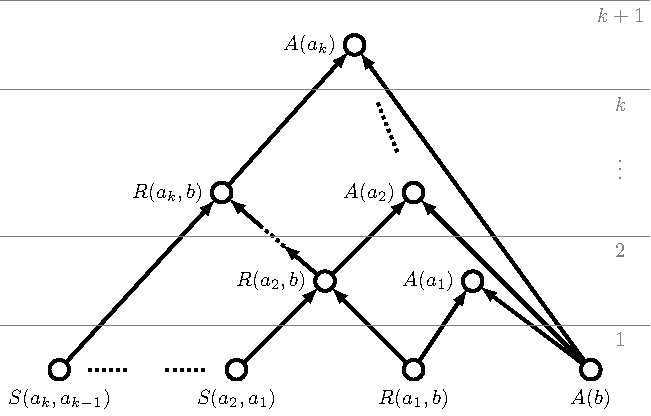
\includegraphics[width=0.7\textwidth]{fig-mg.eps}
\caption{An example of a materialization graph.}
\label{fig:mg}
\end{center}
\end{figure}

We say that a materialization graph $\mathcal{G}$ is a \emph{complete materialization graph}
when $\mathcal{G}$ contains all ground atoms in $T_R^{\omega}(\textbf{I})$.
The set of nodes in a complete materialization graph is actually the result
of materialization.
Thus, the procedure of materialization can be transformed to the construction of
a complete materialization graph.
We pay our attention to complete materialization graphs and do not distinguish it to the
notion `materialization graph'.
It should also be noted that there may exist several materialization graphs for a datalog program.


\subsection{A Basic Parallel Algorithm}

In this part, we propose a parallel algorithm
(denoted by Algorithm~$\mathsf{A}_{bsc}$) that constructs a materialization graph for a given datalog program.
Our computational model is a PRAM (parallel, random-access machine) that is mostly used to analyze the parallel
complexity. This model allows us giving \emph{the parallel assumption}: 
for any datalog program $P=\langle R, \textbf{I}\rangle$,
any substitution of some atom and any rule instance in $P^*$ can be mapped to a unique memory
location; further, a one-to-one relation can be established between processors and rule instances.
Under this assumption, a processor can check the applicability of its corresponding
rule instance and access the state of an atom occurring in this rule instance in constant time.
Algorithm~$\mathsf{A}_{bsc}$ is then given as follows.\\


\noindent\texttt{Algorithm~$\mathsf{A}_{bsc}$}. Given a datalog program $P=\langle R, \textbf{I}\rangle$,
the algorithm returns a materialization graph $\mathcal{G}$ of $P$.
Suppose we have $|P^*|$ processors, and each rule instantiation in $P^*$ is
assigned to one processor.
Initially $\mathcal{G}$ is empty. The following three steps are then performed:
\begin{enumerate}[leftmargin=8ex,label=(\textit{Step \arabic*}),ref=Step~\arabic*]
\item Add all facts in $\textbf{I}$ to $\mathcal{G}$.\label{alg1:addFacts}
\item For each rule instantiation $B_1,...,B_n\rightarrow H$, if the body atoms are all
    in $\mathcal{G}$ while $H$ is not in $\mathcal{G}$,\footnote{Suppose that each processor
    can use $O(1)$ time units to access the state of ground atoms, i.e., whether this ground
    atom has been added to the materialization graph. This can be implemented by maintaining an
    index of polynomial size.}
    the corresponding processor adds $H$ to $\mathcal{G}$ and creates edges pointing
    from $B_1,...,B_n$ to $H$.\label{alg1:updateG}
\item If no processor can add more nodes and edges to $\mathcal{G}$, terminate, otherwise iterate \ref{alg1:updateG}.\label{alg1:halt}\hfill$\Box$
\end{enumerate}

\begin{example}
We consider the datalog program $P_{ex_1}$ in Example~\ref{exp:mg} again,
and perform Algorithm~$\mathsf{A}_{bsc}$ on it.
Initially, all the facts ($A(b),R(a_1,b),S(a_2,a_1),...,S(a_{k},a_{k-1})$) are added to the
result $\mathcal{G}_{ex_1}$ (\ref{alg1:addFacts}).
Then in different iterations of \ref{alg1:updateG}, the remaining nodes are added to
$\mathcal{G}_{ex_1}$ by different processors.
For example a processor $p$ is allocated a rule instantiation `$R(a_2,b),A(b)\rightarrow A(a_2)$'.
Then, processor $p$ adds $A(a_2)$ to $\mathcal{G}_{ex_1}$ after it checks that
$A(b)$ and $R(a_2,b)$ are in $\mathcal{G}_{ex_1}$.
Algorithm~$\mathsf{A}_{bsc}$ halts when $A(a_k)$ has been added to $\mathcal{G}_{ex_1}$ (\ref{alg1:halt}).
\end{example}

Lemma~\ref{lemma:a1} shows the correctness of Algorithm~$\mathsf{A}_{bsc}$ and that, for any datalog program $P$,
Algorithm~$\mathsf{A}_{bsc}$ always constructs a materialization graph with the minimum depth among all the
materialization graphs of $P$. The detailed proofs of Lemma~\ref{lemma:a1} and other lemmas and theorems can be found
in the appendix.

\begin{lemma}
\label{lemma:a1}
Given a datalog program $P=\langle R, \textbf{I}\rangle$, we have
\begin{enumerate}[leftmargin=4ex]
\item Algorithm~$\mathsf{A}_{bsc}$ halts and returns a materialization graph $\mathcal{G}$ of $P$;
\item $\mathcal{G}$ has the the minimum depth among all the materialization graphs of $P$.
\end{enumerate}
\end{lemma}

\begin{proof}[Proof sketch] This lemma can be proved by performing
an induction on $T_R^{\omega}(\textbf{I})$.
The stage (see the related contents in Section~\ref{sec:background}) of $P$
is the lower-bound of the depth of the materialization graphs. Based on the previous induction,
one can further check that, for the materialization graph $\mathcal{G}$ constructed by Algorithm~$\mathsf{A}_{bsc}$,
its depth equals the depth of the stage.
\end{proof}

We now discuss the parallel complexity of Algorithm~$\mathsf{A}_{bsc}$.
Given a class of datalog programs $\mathbb{P}$ where
a rule set is shared for each datalog program $P=\langle R, \textbf{I}\rangle$ in $\mathbb{P}$.
Let $e$, $v$ and $r$ represent the maximum arity of any EDB predicate, the maximum number of variables
in any datalog rule, and the number of datalog rules respectively.
We then have that the number of
constants is at most $|\textbf{I}|e$, and the number of all possible rule instances in $P^*$
is at most $r(|\textbf{I}|e)^v$.
Note that $e, v$ and $r$ depend only on the rule set $R$ and not on the fact set $\textbf{I}$.
Thus, the memory space for storing the atoms and the rule instances is polynomial in the size of $\textbf{I}$.
This also means that the number of processors is polynomially bounded.
The computing time of \ref{alg1:addFacts} and \ref{alg1:halt} occupies constant time (denoted by $c_1$) because of parallelism.
Since Algorithm~$\mathsf{A}_{bsc}$ works under the parallel assumption, one iteration of
\ref{alg1:updateG} also costs constant time (denoted by $c_2$). Thus, 
the whole computing time of Algorithm~$\mathsf{A}_{bsc}$ turns out to be $c_1+l\cdot c_2$
where $l$ denotes the number of iterations of \ref{alg1:updateG}.

When we say that an algorithm is an NC algorithm. It should meet two requirements: first,
it works on a polynomial number of processors; second, it halts in poly-logarithmic time.
As discussed above, Algorithm~$\mathsf{A}_{bsc}$ meets the first requirement.
If we want to restrict Algorithm~$\mathsf{A}_{bsc}$ to be an NC algorithm,
we can make the number of iterations of \ref{alg1:updateG} to be poly-logarithmically bounded.
We use the symbol $\psi$ to denote a poly-logarithmically bounded function.
For any datalog program, if we restrict that the number of iterations of \ref{alg1:updateG} is bounded by $\psi(|\textbf{I}|)$, 
the computing time of Algorithm~$\mathsf{A}_{bsc}$
is $c_1+\psi(|\textbf{I}|)\cdot c_2$. With this restriction, Algorithm~$\mathsf{A}_{bsc}$ is an NC algorithm denoted by
$\mathsf{A}_{bsc}^{\psi}$.

Based on $\mathsf{A}_{bsc}^{\psi}$, we can identify a class of datalog programs
$\mathcal{D}_{\mathsf{A}_{bsc}^{\psi}}$ such that all the datalog programs in it can be handled
by $\mathsf{A}_{bsc}^{\psi}$.
It is obvious that $\mathcal{D}_{\mathsf{A}_{bsc}^{\psi}}$ is a \texttt{PTD} class.
We use the following theorem to further show that this class can be captured based on
the materialization graphs of the datalog programs in $\mathcal{D}_{\mathsf{A}_{bsc}^{\psi}}$.

\begin{theorem}\label{theorem:a1}
For any datalog program $P$, $P\in\mathcal{D}_{\mathsf{A}_{bsc}^{\psi}}$ iff $P$ has a
materialization graph whose depth is upper-bounded by $\psi(|P|)$.
\end{theorem}

\begin{proof}[Proof sketch]
We can first prove that the number of iterations
of \ref{alg1:updateG} is actually the depth of the constructed materialization
graph. This theorem then follows by considering
Lemma~\ref{lemma:a1}.
\end{proof}

Consider Example~\ref{exp:mg} again. Let the integer $k$ be a variable. We can
get a class of datalog programs, denoted by $\mathbb{P}_{ex_1}$, where the rule set
is $\{R(x,y),A(y)\rightarrow A(x), S(x,y),R(y,z)\rightarrow R(x,z)\}$ and the fact
set varies according to $k$. The algorithm $\mathsf{A}_{bsc}^{\psi}$ is restricted in the sense that it cannot even work on the rather simple datalog program class $\mathbb{P}_{ex_1}$.
It can be checked that, for some materialization graph $\mathcal{G}_{ex_1}$
corresponding to a datalog program in $\mathbb{P}_{ex_1}$, \texttt{depth}($\mathcal{G}_{ex_1}$)$=k$ for some $k$.
This means that the depths of the materialization graphs are linearly bounded by $k$.
On the other hand, the sizes of the datalog programs in $\mathbb{P}_{ex_1}$ are polynomial of $k$.
Thus, for any $\psi$ that is poly-logarithmically bounded, we can always find a $k$ large
enough such that $\mathsf{A}_{bsc}^{\psi}$ terminates without constructing a materialization
graph for each datalog program in $\mathbb{P}_{ex_1}$.
However there indeed exists an NC algorithm that can handle $\mathbb{P}_{ex_1}$.
We discuss this in the next part.


\subsection{Optimizing Algorithm~$\mathsf{A}_{bsc}$ via the Single-Way Derivability}

In this part, we optimize Algorithm~$\mathsf{A}_{bsc}$ such that $P_{ex_1}$
can be handled. Based on the optimized variant of Algorithm~$\mathsf{A}_{bsc}$,
we can identify another \texttt{PTD} class.

We discuss our optimization based on a specific case in Example~\ref{exp:general}.
We find that, in this kind of case, the construction of a materialization graph can be accelerated.

\begin{figure}[htbp]
\begin{center}
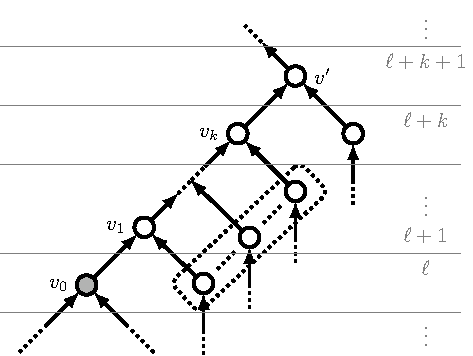
\includegraphics[width=0.7\textwidth]{fig-general.eps}
\caption{A partial materialization graph.}
\label{fig:general}
\end{center}
\end{figure}

\begin{example}\label{exp:general}
Consider a snapshot of Algorithm~$\mathsf{A}_{bsc}$ in
Figure~\ref{fig:general}. A materialization graph $\mathcal{G}$
is being constructed for some datalog program $\langle R, \textbf{I}\rangle$.
The nodes in the dashed box denote the ones that have been added to $\mathcal{G}$.
In this snapshot, $v_0$ has been newly added
to $\mathcal{G}$ in the $l^{th}$ ($l\geq 1$) iteration.
Each of the nodes $v_i$ ($1\leq i\leq k$) has almost one parent node being not in $\mathcal{G}$,
while $v'$ has two parent nodes being not in $\mathcal{G}$.
All of the nodes $v_i$ ($1\leq i\leq k$) and $v'$ would be added to $\mathcal{G}$
afterwards.
\end{example}


In Example~\ref{exp:general}, $v_k$ would be added to $\mathcal{G}$ after \emph{at least} $k$
iterations by performing Algorithm~$\mathsf{A}_{bsc}$.
We can check that each edge $(v_{i-1},v_i)$ ($1\leq i\leq k$) in this stage follows the condition:
\emph{if the parent node $v_{i-1}$ is derivable, the child node $v_i$ has to be derivable} (this
is because that, for node $v_i$, node $v_{i-1}$ is the only parent node that has not been added to $\mathcal{G}$).
We call this condition \emph{the single-way derivability condition}, which intuitively says that the derivability of a
node only depends on one of its parent nodes.
Observe that node $v_k$ is reachable from node $v_0$ through the path $\tau=(v_0,v_1,...,v_k)$ where
each edge $(v_{i-1},v_i)$ ($1\leq i\leq k$) follows the single-way derivability condition;
we call such a path a \emph{single-way derivable} (SWD) path.
Further, the starting node $v_0$ in $\tau$ has been added to $\mathcal{G}$; in other words,
$v_0$ is derivable. Thus, all of the nodes $v_i$ ($1\leq i\leq k$) can be added to
$\mathcal{G}$ immediately.
Based on the above idea, we optimize Algorithm~$\mathsf{A}_{bsc}$ by checking whether such an SWD path
exits for some node $v$; if there is an SWD path for node $v$, this node can be added to $\mathcal{G}$
due to the single-way derivability condition.

Backing to Example~\ref{exp:general}, since
there exists an SWD path $(v_0,...,v_i)$ for each node $v_i$ ($1\leq i\leq k$), all of these nodes
can be added to $\mathcal{G}$ right after $v_0$. On the other hand,
node $v'$ has no SWD path, since it has two parent nodes being not in $\mathcal{G}$.

We next discuss how to determine the existence of SWD paths. Note that, SWD paths require us to
describe the reachability between two nodes. To this extent, we use a
binary transitive relation $\texttt{rch} \subseteq T_R^{\omega}(\textbf{I})\times T_R^{\omega}(\textbf{I})$,
e.g., \texttt{rch}$(v_1,v_2)$ means that $v_2$ is reachable from $v_1$.
In each iteration of \ref{alg1:updateG} in Algorithm~$\mathsf{A}_{bsc}$, we further compute a \texttt{rch}
relation (denoted by $S_{\textit{\tiny rch}}$) by performing the following process:

\begin{description}[leftmargin=2ex]
\item[(\textbf{\dag})] \emph{For each rule instantiation of the form $B_1,..,B_i,..,B_n\rightarrow H$
where $H$ has not been added to $\mathcal{G}$}:
\begin{enumerate}[leftmargin=2ex]
\item \emph{if the body atoms $B_1,...,B_n$ have all been added to $\mathcal{G}$, put \texttt{rch}$(B_1,H),...,$ \texttt{rch}$(B_n,H)$ in $S_{\textit{\tiny rch}}$};
\item \emph{if $B_i$ is the only node in the body that has not been added to $\mathcal{G}$,
    put \texttt{rch}$(B_i,H)$ in $S_{\textit{\tiny rch}}$}.\hfill$\Box$
\end{enumerate}
\end{description}

We then compute the transitive closure (denoted by $S^*_{\textit{\tiny rch}}$) with respect to
$S_{\textit{\tiny rch}}$. Based on the transitive closure, we can perform the optimization that,
for a node $v$, if there is a relation $\texttt{rch}(v',v)\in S^*_{\textit{\tiny rch}}$
where $v'$ has been added to $\mathcal{G}$, $v$ has an SWD path and can be added to $\mathcal{G}$.
The following algorithm applies this optimization strategy.\\

\noindent\texttt{Algorithm~$\mathsf{OPT}$}. The algorithm requires two inputs:
a datalog program $P=\langle R, \textbf{I}\rangle$ and a (partial) materialization graph $\mathcal{G}$ that is
being constructed from $P$. The following steps are performed:
\begin{enumerate}[leftmargin=6ex,label=(\textbf{\roman*})]
\item Compute a \texttt{rch} relation $S_{\textit{\tiny rch}}$ by following the above process (see $(\textbf{\dag})$).\label{rch}
\item Compute the transitive closure $S^*_{\textit{\tiny rch}}$ of $S_{\textit{\tiny rch}}$.\label{transClos}
\item Update $\mathcal{G}$ as follows: for any \texttt{rch}$(B_i,H)\in S_{\textit{\tiny rch}}$
that corresponds to `$B_1,..,B_i,..$ $,B_n\rightarrow H$'
    and there exists a node $B'$ such that \texttt{rch}$(B',B_i)\in S^*_{\textit{\tiny rch}}$ and $B'$ is
    in $\mathcal{G}$; if $H$ is not in $\mathcal{G}$ or $H$ is in $\mathcal{G}$ but has no parent pointing
    to it, add $H$ and $B_i$ (if $B_i$ is not in $\mathcal{G}$) to $\mathcal{G}$, and create the edges
    $e(B_1, H),...,e(B_n, H)$ in $\mathcal{G}$. Do nothing for other statements
    \texttt{rch}$(B_j,H)\in S_{\textit{\tiny rch}}$.\label{updateG}\hfill$\Box$
\end{enumerate}

It is well known that there is an NC algorithm for computing the
transitive closure \cite{Allender07}.
Based on this result and Algorithm~$\mathsf{OPT}$, we propose an optimized variant of Algorithm~$\mathsf{A}_{bsc}$:\\

\noindent\texttt{Algorithm~$\mathsf{A}_{opt}$}. Given a datalog program $P=\langle R, \textbf{I}\rangle$, the algorithm
returns a materialization graph $\mathcal{G}$ of $P$. Initially $\mathcal{G}$ is empty. The following steps are then performed:
\begin{enumerate}[leftmargin=8ex,label=(\textit{Step \arabic*}),ref=Step~\arabic*]
\item Add all facts in $\textbf{I}$ to $\mathcal{G}$.\label{alg3:addFacts}
\item Compute $S_{\textit{\tiny rch}}$ by performing \ref{rch} in Algorithm~$\mathsf{OPT}$; use an NC
    algorithm to compute the transitive closure $S^*_{\textit{\tiny rch}}$ (see \ref{transClos} in Algorithm~$\mathsf{OPT}$);
    update $\mathcal{G}$ by performing \ref{updateG}  in Algorithm~$\mathsf{OPT}$.\label{alg3:updateG}
\item If no node has been added to $\mathcal{G}$ (in \ref{alg3:updateG}), terminate,
    otherwise iterate \ref{alg3:updateG}. \label{alg3:halt}\hfill$\Box$
\end{enumerate}

It should be noted that there has to be an SWD path for any derivable node in some iteration when performing
Algorithm~$\mathsf{A}_{opt}$.
The following lemma shows the correctness of Algorithm~$\mathsf{A}_{opt}$.

\begin{lemma}\label{lemma:a3}
Given a datalog program $P=\langle R, \textbf{I}\rangle$,
$\mathsf{A}_{opt}$ halts and outputs a materialization graph $\mathcal{G}$ of $P$.
\end{lemma}

\begin{example}\label{exp:opt}
We perform Algorithm~$\mathsf{A}_{opt}$ on the datalog program $P_{ex_1}$ in Example~\ref{exp:mg}.
Initially, $R(a_1,b)$ is in the materialization graph $\mathcal{G}_{ex_1}$.
In the first iteration of \ref{alg3:updateG}, all the rule instantiations are in two kinds of forms:
`$R(a_i,b),A(b)\rightarrow A(a_i)$' and `$S(a_i,a_{i-1}),$ $R(a_{i-1},b)\rightarrow R(a_i,b)$' $(2\leq i\leq k)$,
$S_{\textit{\tiny rch}}$ is the set $\{$\texttt{rch}$(R(a_{i-1},b), R(a_i,b))|2\leq i\leq k\}
\cup\{$\texttt{rch}$(R(a_i,b), A(a_i))|1\leq i\leq k\}$.
In the transitive closure of $S_{\textit{\tiny rch}}$,
one can check that \texttt{rch}$(R(a_1,b), R(a_i,b)),$
\texttt{rch}$(R(a_1,b), A(a_i))\in S^*_{\textit{\tiny rch}}(2\leq i\leq k)$.
Thus, $R(a_i,b)$ and $A(a_i)$ ($2\leq i\leq k$) can all be added to $\mathcal{G}_{ex_1}$
in the first iteration of \ref{alg3:updateG}.
\end{example}

We obtain an NC variant of $\mathsf{A}_{opt}$ analogously to the process for Algorithm~$\mathsf{A}_{bsc}$.
It can be checked that an iteration of \ref{alg3:updateG} in $\mathsf{A}_{opt}$ costs poly-logarithmic
time, since the main part is computing $S^*_{\textit{\tiny rch}}$ by an NC algorithm.
Thus, if the number of iterations of \ref{alg3:updateG} is upper-bounded by a poly-logarithmical function,
$\mathsf{A}_{opt}$ is an NC algorithm.
Analogously to $\mathsf{A}_{bsc}^{\psi}$, we use $\mathsf{A}_{opt}^{\psi}$ to denote an NC variant.
Specifically, for any datalog program $P$, the number of iterations of \ref{alg3:updateG} in $\mathsf{A}_{opt}$
is bounded by $\psi(|P|)$, where $\psi$ is a poly-logarithmically bounded function.

Based on $\mathsf{A}_{opt}^{\psi}$, we can identify a \texttt{PTD} class $\mathcal{D}_{\mathsf{A}_{opt}^{\psi}}$.
Further, we have the following corollary which implies that $\mathsf{A}_{opt}^{\psi}$ performs better
than $\mathsf{A}_{bsc}^{\psi}$ in terms of computing time.

\begin{corollary}
For any poly-logarithmically bounded function $\psi$,
we have that $\mathcal{D}_{\mathsf{A}_{bsc}^{\psi}}\subseteq\mathcal{D}_{\mathsf{A}_{opt}^{\psi}}$.
\end{corollary}

\begin{proof}[Proof sketch]
Suppose $P\in\mathcal{D}_{\mathsf{A}_{bsc}^{\psi}}$. According to Theorem~\ref{theorem:a1},
the depth of the materialization graph $\mathcal{G}$ constructed by $\mathsf{A}_{bsc}^{\psi}$ is upper-bounded by $\psi(|P|)$.
It is obvious that the number of nodes in each path of $\mathcal{G}$ is also upper-bounded by $\psi(|P|)$.
According to the optimization strategy applied in $\mathsf{A}_{opt}$, if $\mathcal{G}$ can be constructed
by $\mathsf{A}_{opt}$, the number of iterations of $\mathsf{A}_{opt}$ has to be upper-bounded by $\psi(|P|)$;
if $\mathcal{G}$ is not the materialization graph constructed
by $\mathsf{A}_{opt}$, then there has to exist another materialization graph $\mathcal{G}'$ constructed by $\mathsf{A}_{opt}$
and $\mathcal{G}'$ has a smaller depth compared with $\mathcal{G}$.
\end{proof}


\section{Parallel Tractability of Ontology Materialization in OWL}
\label{sec:ptonto}

In this section, we study the issue of parallel tractability
for materialization of DL-Lite and DHL (DHL($\circ$)) ontologies
based on Algorithm~$\mathsf{A}_{opt}$.
We show that, for any DL-Lite$_{core}$ or DL-Lite$_\mathcal{R}$ ontology $\mathcal{O}$,
there exists a poly-logarithmically bounded function $\psi$
such that Algorithm~$\mathsf{A}_{opt}^{\psi}$ can handle materialization of $\mathcal{O}$.
However, for DHL and DHL($\circ$), there exist ontology classes such that Algorithm~$\mathsf{A}_{opt}^\psi$
does not work. We illustrate the reason why Algorithm~$\mathsf{A}_{opt}^\psi$ cannot always
work by studying specific cases.
Further, we propose to restrict the usage of DHL and DHL($\circ$) in order to achieve parallel tractability
of materialization.

\subsection{Materialization of DL-Lite Ontologies via Algorithm~$\mathsf{A}_{opt}$}

In this part, we show how to use Algorithm~$\mathsf{A}_{opt}$ to handle
DL-Lite materialization and analyze its parallel tractability.
Based on the analysis, we have that, for any DL-Lite$_{core}$ or DL-Lite$_\mathcal{R}$ ontology
there always exists an SWD path for each atom of the form $A(a)$ or $R(a,b)$.
In other words, all atoms of the forms $A(a)$ and $R(a,b)$ can be added to
the constructed materialization graph in the first iteration of \ref{alg3:updateG}
by performing Algorithm~$\mathsf{A}_{opt}$.

In order to show how Algorithm~$\mathsf{A}_{opt}$ handles DL-Lite materialization,
we use the following example.

\begin{example}\label{exp:dllite}
Given a DL-Lite ontology $\mathcal{O}_{ex_5}$
where its TBox and RBox contain the following axioms:
$A\sqsubseteq B_1$, $A\sqsubseteq B_2$, $B_1\sqcap B_2\sqsubseteq\bot$,
$\exists R.B_2\sqsubseteq\bot$, $Q\sqsubseteq S^-$, $S\sqsubseteq R$;
its ABox contains an assertion $Q(a,b)$.
We denote the corresponding datalog program of $\mathcal{O}_{ex_5}$ by $P_{ex_5}=\langle R, \textbf{I}\rangle$,
where $R$ contains the rules that are transformed from the above axioms; $\textbf{I}$ contains $Q(a,b)$
as the only fact.
The unique materialization graph of $P_{ex_5}$ is denoted by $\mathcal{G}_{ex_5}$ (see Figure~\ref{fig:ex2}).
\end{example}

\begin{figure}[htbp]
\begin{center}
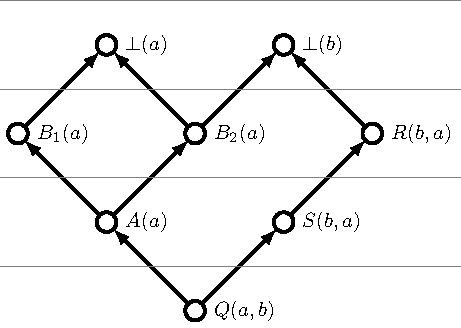
\includegraphics[width=0.6\textwidth]{fig-dllite.eps}
\caption{The materialization graph of $\mathcal{O}_{ex_5}$.}
\label{fig:ex2}
\end{center}
\end{figure}

Consider performing Algorithm~$\mathsf{A}_{opt}$ on the ontology $\mathcal{O}_{ex_5}$ in Example~\ref{exp:dllite}.
(\uppercase\expandafter{\romannumeral1}) First, Algorithm~$\mathsf{A}_{opt}$ adds all ABox assertions (only $Q(a,b)$ here)
to $\mathcal{G}_{ex_5}$ that is initially an empty graph (\ref{alg3:addFacts} of Algorithm~$\mathsf{A}_{opt}$).
(\uppercase\expandafter{\romannumeral2}) In the first iteration of
\ref{alg3:updateG}, Algorithm~$\mathsf{A}_{opt}$ checks that all of the nodes
$A(a)$, $S(b,a)$, $B_1(a)$, $B_2(a)$ and $R(b,a)$ have corresponding SWD paths
starting from $Q(a,b)$. Thus, Algorithm~$\mathsf{A}_{opt}$
adds these nodes to $\mathcal{G}_{ex_5}$ immediately. We take an example of node $B_1(a)$,
for which an SWD path $(Q(a,b),A(a),B_1(a))$ exists.
When updating $\mathcal{G}_{ex_5}$ by adding $B_1(a)$ to it,
Algorithm~$\mathsf{A}_{opt}$ first checks whether the parent node $A(a)$ of $B_1(a)$
has been in $\mathcal{G}_{ex_5}$; if $A(a)$ is already in $\mathcal{G}_{ex_5}$, $B_1(a)$
is added to $\mathcal{G}_{ex_5}$ by creating an edge pointing from $A(a)$ to $B_1(a)$;
if $A(a)$ has not been added to $\mathcal{G}_{ex_5}$, Algorithm~$\mathsf{A}_{opt}$ adds $A(a)$ (resp., $B_1(a)$)
to $\mathcal{G}_{ex_5}$ and creates an edge pointing from $Q(a,b)$ to $A(a)$ (resp.,
an edge pointing from $A(a)$ to $B_1(a)$).\footnote{These two cases may happen simultaneously,
since node $A(a)$ and node $B_1(a)$ are being processed in parallel.} The other nodes
$A(a)$, $S(b,a)$, $B_2(a)$ and $R(b,a)$ are processed similarly.
(\uppercase\expandafter{\romannumeral3})
The two nodes $\bot(a)$ and $\bot(b)$
have no SWD path in the first iteration of \ref{alg3:updateG}.
They are left to be processed in the second iteration.
(\uppercase\expandafter{\romannumeral4})
Finally, Algorithm~$\mathsf{A}_{opt}$ finishes constructing $\mathcal{G}_{ex_5}$
after two iterations (\ref{alg3:halt}).

From the above example, we can observe that SWD paths exist
for all nodes except $\bot(a)$ and $\bot(b)$ in the first iteration of Algorithm~$\mathsf{A}_{opt}$.
Further, we give the following lemma that satisfies any DL-Lite$_{core}$ or DL-Lite$_\mathcal{R}$ ontology.

\begin{lemma}\label{lemma:dllite}
For any DL-Lite$_{core}$ or DL-Lite$_\mathcal{R}$ ontology $\mathcal{O}$, there exists a materialization graph $\mathcal{G}$ such that
each atom of the form $A(x)$ ($A\neq\bot$) or $R(x,y)$ in $\mathcal{G}$ has an SWD path.
\end{lemma}

The above lemma guarantees that all atoms of the form $A(x)$ ($A\neq\bot$) or $R(x,y)$
have to be added to the constructed materialization graph in the first iteration of
\ref{alg3:updateG} by applying Algorithm~$\mathsf{A}_{opt}$.
For each atom of the form $\bot(x)$, there may not exist an SWD path in the first iteration
of \ref{alg3:updateG}, since its derivability depends on its two parent nodes
(see nodes $\bot(a)$ and $\bot(b)$ in $\mathcal{G}_{ex_5}$ of
Example~\ref{exp:dllite}). On the other hand, according to the syntaxes of DL-Lite,
$\bot$ dose not occur on the left hand of any axiom. In other words,
an atom of the form $\bot(x)$ cannot be the parent of any other node.
This allows all atoms of the form $\bot(x)$ being added
to the constructed materialization graph in at most two iterations of
\ref{alg3:updateG} by applying Algorithm~$\mathsf{A}_{opt}$.
Based on the above discussion, for any DL-Lite ontology $\mathcal{O}$,
there always exists a poly-logarithmically bounded function $\psi$ such that
Algorithm~$\mathsf{A}_{opt}^{\psi}$ can handle the materialization of $\mathcal{O}$;
more precisely, we can set that $\psi=2$. This result is consistent with
that in \cite{CalvaneseGLLR07}.
Formally, we use $\mathcal{D}_{\textit{\text{dl\_lite}}}$
to denote the set of all DL-Lite$_{core}$ and DL-Lite$_\mathcal{R}$ ontologies, and give the following theorem.

\begin{theorem}\label{theorem:dl-lite}
There exists a poly-logarithmically bounded function $\psi$ s.t.
$\mathcal{D}_{\textit{\text{dl\_lite}}}\subseteq\mathcal{D}_{\mathsf{A}_{opt}^{\psi}}$.
\end{theorem}


\subsection{Parallelly Tractable Materialization of DHL}

In this part, we study whether Algorithm~$\mathsf{A}_{opt}^\psi$ can handle DHL ontologies.
Unfortunately there exist DHL ontology classes such that Algorithm~$\mathsf{A}_{opt}^\psi$
does not work for any poly-logarithmically bounded function $\psi$.
In the following, we first give such a case
to illustrate the reason why Algorithm~$\mathsf{A}_{opt}^\psi$ cannot work.
Based on the analysis of this case, we propose to restrict
the usage of DHL in order to achieve parallel tractability
of materialization.

We find that, an unlimited usage of axioms of the
form $B_1\sqcap B_2\sqsubseteq A$
makes it impossible for Algorithm~$\mathsf{A}_{opt}$ to construct a materialization graph
in a poly-logarithmical number of iterations of \ref{alg3:updateG}.
We use the following example to illustrate it.

\begin{figure}[htbp]
\begin{center}
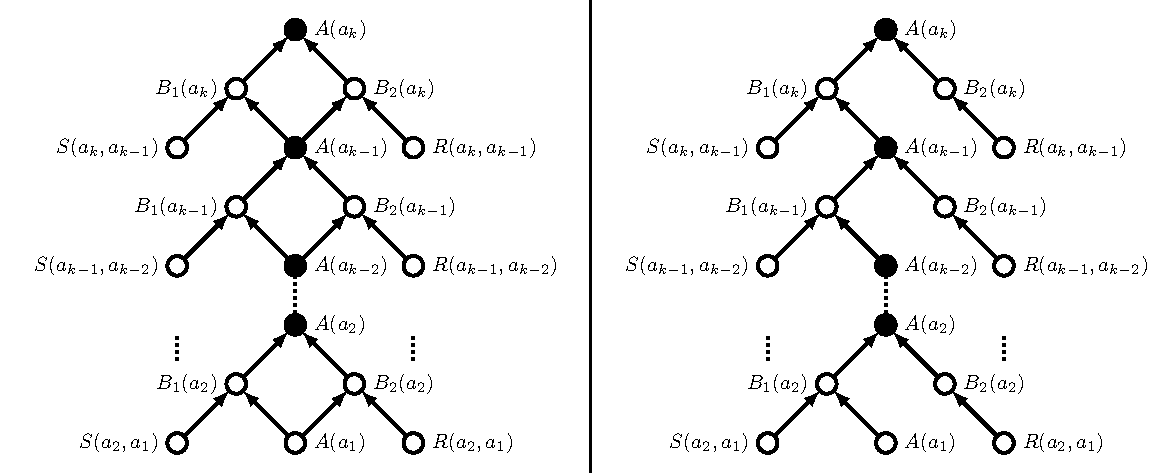
\includegraphics[width=0.9\textwidth]{fig-pathtwist.eps}
\caption{(left) The materialization graph of $\mathcal{O}_{ex_6}$;
(right) The materialization graph of $\mathcal{O}_{ex_7}$.}
\label{fig:ex3_4}
\end{center}
\end{figure}

\begin{example}\label{exp:dhl}
Given a DHL ontology $\mathcal{O}_{ex_6}$ where its TBox contains three axioms:
$B_1\sqcap B_2\sqsubseteq A$, $\exists S.A\sqsubseteq B_1$ and $\exists R.A\sqsubseteq B_2$;
the ABox is $\{S(a_i,a_{i-1}), R(a_i,a_{i-1}), A(a_1)\}$
for $2\leq i\leq k$ and $k$ is an integer greater than 2.
We denote the corresponding datalog program of $\mathcal{O}_{ex_6}$ by $P_{ex_6}=\langle R, \textbf{I}\rangle$,
where $R$ contains three rules: `$B_1(x),B_2(x)\rightarrow A(x)$',`$S(x,y),A(y)\rightarrow B_1(x)$' and `$R(x,y),A(y)\rightarrow B_2(x)$'.
The materialization graph of $P_{ex_6}$ constructed by $\mathsf{A}_{opt}$ is denoted by $\mathcal{G}_{ex_6}$ (see Figure~\ref{fig:ex3_4}(left)).
\end{example}

One can check that $\mathcal{G}_{ex_6}$ is the unique materialization graph of $P_{ex_6}$.
Observe that there exists a path (e.g., $A(a_1),B_1(a_2),A(a_2),...,A(a_k)$) between $A(a_1)$ and $A(a_k)$.
When performing Algorithm~$\mathsf{A}_{opt}$ on $P_{ex_6}$, it can be checked that
each node of the form $A(a_i)$ (filled with black color,
and $2\leq i\leq k$) has no SWD path until the $i^{th}$ iteration;
in the $i^{th}$ iteration, the parent nodes of $A(a_i)$ have been added to $\mathcal{G}_{ex_6}$,
and, $A(a_i)$ can also be added to $\mathcal{G}_{ex_6}$.
Similar to the datalog program class $\mathbb{P}_{ex_1}$, we can also get a
datalog program class $\mathbb{P}_{ex_6}$ for the ontology $\mathcal{O}_{ex_6}$
when $k$ is a variable. Based on the above analysis, Algorithm~$\mathsf{A}_{opt}$ cannot complete the materialization
for the datalog programs of $\mathbb{P}_{ex_6}$ in a poly-logarithmical
number of iterations.
The intuitive reason is that, at least two paths exist
starting from $A(a_1)$ to $A(a_k)$. These paths \emph{twist} mutually and share the same joint nodes (see the black nodes).
It makes the optimization of acceleration used in Algorithm~$\mathsf{A}_{opt}$ invalid.
That is, for each node $A(a_i)$ ($2\leq i\leq k$), until its parents ($B_1(a_i)$ and $B_2(a_i)$) are added
to $\mathcal{G}_{ex_6}$, there would not exist an available SWD path for $A(a_i)$.
We use `\emph{path twisting}' to represent such cases.

In order to make Algorithm~$\mathsf{A}_{opt}$ terminate in a poly-logarithmical number of iterations,
we consider restricting the usage of axioms of the form $B_1\sqcap B_2\sqsubseteq A$
to avoid `path twisting'. An intuitive idea is to
ensure that \emph{there is only one path between each two atoms of the form $A(x)$
generated from the rules corresponding to (T1)}.
We explain it by using the following example where the ontology is modified from
that in Example~\ref{exp:dhl}.

\begin{example}\label{exp:simpleC}
Consider an ontology $\mathcal{O}_{ex_7}$ where the TBox contains three axioms:
$B_1\sqcap B_2\sqsubseteq A$, $\exists S.A\sqsubseteq B_1$ and $B_3\sqsubseteq B_2$;
the ABox is $\{S(a_i,a_{i-1}), B_3(a_i), A(a_1)\}$
for $2\leq i\leq k$ and $k$ is an integer greater than 2.
We denote the corresponding datalog program by $P_{ex_7}$ where the rule set contains:
`$B_1(x),B_2(x)\rightarrow A(x)$',`$S(x,y),A(y)\rightarrow B_1(x)$' and `$B_3(x)\rightarrow B_2(x)$'.
$P_{ex_7}$ has a unique materialization graph denoted by $\mathcal{G}_{ex_7}$ (see Figure~\ref{fig:ex3_4}(right)).
\end{example}

In the above example, for the axiom $B_1\sqcap B_2\sqsubseteq A$, all derived atoms
of the form $B_2(x)$ must not be child nodes of an atom $A(y)$ for some $y$.
This ensures that only one path exists between each two nodes among $A(a_2),...,A(a_k)$.
Further, when constructing $\mathcal{G}_{ex_7}$, Algorithm~$\mathsf{A}_{opt}$ can terminate after
two iterations of \ref{alg3:updateG}. Specifically, in the first iteration, Algorithm~$\mathsf{A}_{opt}$
adds all of the nodes $B_3(a_i)$ and $B_2(a_i)$ ($2\leq i\leq k$) to $\mathcal{G}_{ex_7}$,
since they have corresponding SWD paths;
after that, all the other nodes
can be added to $\mathcal{G}_{ex_7}$ in the second iteration (because each
node has an SWD path).
Motivated by this example, we consider restricting the usage of
the axioms $B_1\sqcap B_2\sqsubseteq A$
such that all atoms of the form $B_1(x)$ or $B_2(x)$ cannot be generated by an atom $A(y)$
for some $y$.
To this end, we first define \emph{simple concepts} as follows:

\begin{definition}
Given an ontology $\mathcal{O}=\langle\mathcal{T},\mathcal{R},\mathcal{A}\rangle$,
a concept $A\in\textbf{CN}$ is simple, if (1) $A$ does not occur on the right-hand side
of some axiom; or (2) $A$ satisfies the following conditions:
\begin{enumerate}[leftmargin=4ex,label=\arabic*.]
\item for each $B\sqsubseteq A\in\mathcal{T}$, $B$ is simple;
\item for each $\exists R.B\sqsubseteq A\in\mathcal{T}$, $B$ is simple;
\item there is no axiom of the form $B_1\sqcap B_2\sqsubseteq A$ in $\mathcal{T}$.
\end{enumerate}
\end{definition}

Based on simple concepts, we restrict DHL ontologies such that, in all axioms of the
form $B_1\sqcap B_2\sqsubseteq A$, at least one concept of $B_1$ and $B_2$ should be a simple concept
(we call it \emph{simple-concept restriction}).
Intuitively, for the restricted DHL ontologies, the situation of `path twisting' would not happen.
This is because, if in each axiom of the form $B_1\sqcap B_2\sqsubseteq A$, w.l.o.g., $B_1$
is a simple concept, then none of ancestors of $B_1(x)$ for some $x$
is generated from the rules corresponding to (T1).

\begin{example}
In the ontology of Example~\ref{exp:dhl}, all of $A$, $B_1$ and $B_2$ are
non-simple concepts.
In the ontology of Example~\ref{exp:simpleC}, $A$ and $B_1$ are non-simple concepts,
while $B_3$ and $B_2$ are simple concepts. Further, it can be checked that,
the ontology  of Example~\ref{exp:simpleC} follows the simple-concept restriction
and can be handled by Algorithm~$\mathsf{A}_{opt}^\psi$ for some poly-logarithmical function $\psi$.
\end{example}

We define the following class of DHL ontologies based on the above restriction and
give Theorem \ref{theorem:dhl} to show that any DHL ontology that satisfies the
simple-concept restriction can be handled by Algorithm~$\mathsf{A}^\psi_{opt}$
for some poly-logarithmical function $\psi$.

\begin{definition} Let $\mathcal{D}_{\textit{\text{dhl}}}$ be a class of datalog programs where
each program is rewritten from a DHL ontology that follows the condition that, for all axioms of the form
$A_1\sqcap A_2\sqsubseteq B$, at least one concept of $A_1$ and $A_2$ should be a \emph{simple concept}.
\end{definition}

\begin{theorem}\label{theorem:dhl}
There exists a poly-logarithmically bounded function $\psi$ s.t.
$\mathcal{D}_{\textit{\text{dhl}}}\subseteq\mathcal{D}_{\mathsf{A}_{opt}^{\psi}}$.
\end{theorem}


\subsection{Parallelly Tractable Materialization of DHL($\circ$)}

In this part, we study parallelly tractable materialization
of DHL($\circ$) ontologies.
In addition to the rules in DHL, we also have to consider complex RIAs (R4).
We next show that complex RIAs may also cause the situation of `path twisting'.
Consider the following example.

\begin{example}\label{exp:complexRIA}
Given a DHL$(\circ)$ ontology $\mathcal{O}_{ex_9}$ where its TBox is empty;
the RBox $\mathcal{R}$ contains three axioms:
$R_1\circ R_2\sqsubseteq R$, $R_3\circ R\sqsubseteq R_1$ and $R\circ R_4\sqsubseteq R_2$;
the ABox $\mathcal{A}$ is $\{R(a_1,a_1), R_3(a_i,a_{i-1}), R_4(a_{i-1},a_i)\}$
for $2\leq i\leq k$ and $k$ is an integer greater than 2.
The corresponding datalog program $P_{ex_5}$
contains three rules: `$R_1(x,y),R_2(y,z)\rightarrow R(x,z)$',
`$R_3(x,y),R(y,z)\rightarrow R_1(x,z)$' and `$R(x,y),R_4(y,z)\rightarrow R_2(x,z)$'.
The materialization graph of $P_{ex_5}$ constructed by Algorithm~$\mathsf{A}_{opt}$ is denoted by $\mathcal{G}_{ex_9}$.
\end{example}

One can check that the materialization graph $\mathcal{G}_{ex_9}$ has the same shape as that
of $\mathcal{G}_{ex_6}$ in Figure~\ref{fig:ex3_4}.
A twisted path exists in $\mathcal{G}_{ex_9}$ involving $R(a_i,a_i) (2\leq i\leq k)$ as the joint nodes.
Further, all the roles $R_1$, $R_2$, $R_3$, $R_4$ and $R$ in this example are non-transitive roles.

Inspired by what we do for axioms $B_1\sqcap B_2\sqsubseteq A$,
we require that, for all axioms of the form $R_1\circ R_2\sqsubseteq R$,
if $R$ is not a transitive role and no transitive role $S$ exists such that $R\sqsubseteq_* S$,
then, at least one of $R_1$ and $R_2$ is
a \emph{simple role}.\footnote{See the definition of a simple role in Section~\ref{sec:background}.}
We now consider such an axiom $R_1\circ R_2\sqsubseteq R$ (denoted by $\alpha_1$) where $R$ is a transitive role.
That is we also have $R\circ R\sqsubseteq R$ (denoted by $\alpha_2$).
By replacing $R$ on the left-hand of $\alpha_2$ using $R_1$ and $R_2$,
we can get a complex RIA in the form of
$R_1\circ R_2\circ R_1\circ R_2\sqsubseteq R$ (denoted by $\alpha_3$).
If one of $R_1$ and $R_2$ is not a simple role, the corresponding
rule of $\alpha_3$ may also lead to `path twisting'.\footnote{Obviously, applying the rules of $\alpha_1$
and $\alpha_2$ separately has the same effect to that of only applying the rule of $\alpha_3$.}
The reason can be explained as follows.
Without loss of the generality,
$R_2$ is a simple role while $R_1$ is not.
For some atom $R(x,y)$, it may depend on two different nodes of the predicate $R_1$
through the corresponding rule of $\alpha_3$. The similar analysis applies to
such cases of $\alpha_1$ where $R$ is not a transitive role, while another transitive
role $S$ exists such that $R\sqsubseteq_* S$. That is, we can obtain
a complex RIA of the form $R_1\circ R_2\circ R_1\circ R_2\sqsubseteq S$.
Further, the situation of path twisting also exists.
To tackle the above issue,
we require both of $R_1$ and $R_2$ in $\alpha_1$ to be simple roles
(we call the above restriction for transitive and non-transitive roles \emph{simple-role restriction}).
Combined with the simple-concept restriction,
we define a class of DHL($\circ$) ontologies as follows:

\begin{definition}\label{def:dhlplus}
$\mathcal{D}_{\textit{\text{dhl}}(\circ)}$ is a class of datalog programs where each program
is rewritten from a DHL($\circ$) ontology and the following
conditions are satisfied:
\begin{enumerate}[leftmargin=4ex,label=\arabic*.]
\item for all axioms of the form $A_1\sqcap A_2\sqsubseteq B$,
    at least one concept of $A_1$ and $A_2$ should be a \emph{simple concept};
\item for all axioms of the form $R_1\circ R_2\sqsubseteq R$,
    if there does not exits a transitive role $S$ such that $R\sqsubseteq_* S$, then,
    at least one of $R_1$ and $R_2$ is a \emph{simple role}; otherwise, both of $R_1$ and $R_2$ are \emph{simple roles}.
\end{enumerate}
\end{definition}

\begin{example}
For the ontology $\mathcal{O}_{ex_7}$ in Example~\ref{exp:complexRIA}, all of the roles
$R_1$, $R_2$ and $R$ are non-simple roles. Thus, $\mathcal{O}_{ex_7}$ does not follow
the simple-role restriction because of $R_1\circ R_2\sqsubseteq R$.
Consider the ontology $\mathcal{O}_{ex_1}$
in Example~\ref{exp:mg} again. The role $R$ is a non-simple role, while $S$ is a simple role.
Thus $\mathcal{O}_{ex_1}$ follows the simple-role restriction. All the implicit nodes
in $\mathcal{G}_{ex_1}$ have corresponding SWD paths in the first iteration.
Thus, `path twisting' cannot occur when materializing $\mathcal{O}_{ex_1}$ by Algorithm~$\mathsf{A}_{opt}$.
\end{example}

We further give Theorem~\ref{theorem:dhlplus} to show that Algorithm~$\mathsf{A}_{opt}^{\psi}$ can handle
all the datalog programs in $\mathcal{D}_{\textit{\text{dhl}}(\circ)}$ for some poly-logarithmical function $\psi$.

\begin{theorem}\label{theorem:dhlplus}
There exists a poly-logarithmically bounded function $\psi$ s.t. $\mathcal{D}_{\textit{\text{dhl}}(\circ)}\subseteq\mathcal{D}_{\mathsf{A}_{opt}^{\psi}}$.
\end{theorem}


\section{A Further Optimized Algorithm for DHL$(\circ)$ Materialization}
\label{sec:practicalAlg}

In this section, we first discuss that Algorithm~$\mathsf{A}_{opt}$ can hardly work in practice.
In order to make Algorithm~$\mathsf{A}_{opt}$ more practical,
we propose to modify Algorithm~$\mathsf{A}_{opt}$ and give an algorithm variant Algorithm~$\mathsf{A}_{prc}$.
We show that Algorithm~$\mathsf{A}_{prc}$ can also be restricted to an NC version
when materializing DHL$(\circ)$ ontologies that follow both of the simple-concept
and the role-concept restrictions.

\subsection{Reducing Computing Space}

In previous sections, Algorithm~$\mathsf{A}_{opt}$ is mainly used for theoretical analysis.
However, this algorithm can hardly work in practice due to its inherently
high requirement of computing space. Specifically,
Algorithm~$\mathsf{A}_{opt}$ constructs a materialization graph by checking all possible rule
instantiations in $P^*$ where $P$ is a datalog program that corresponds to an ontology.
One can check that $|P^*|$ could be the square or cube of the number of constants occurring in $P$.
Consider a datalog rule of the form `$R(x,y),A(y)\rightarrow B(x)$'
that is rewritten from the axiom of the form $\exists R.A\sqsubseteq B$;
since there are two variables in this rule, the number of all possible rule instantiations
is $|\textbf{IN}|^2$; if there are
1000 individuals in \textbf{IN}, this number is 1 million.
Similarly, for a datalog rule rewritten from an axiom of the form (R3) or (R4),
the number of all possible rule instantiations is $|\textbf{IN}|^3$.
It is no doubt that a plain implementation of Algorithm~$\mathsf{A}_{opt}$ would be delayed
when the target datalog program or ontology
tends to be large in size.
On the other hand, from Examples~\ref{exp:mg}, \ref{exp:dllite} and \ref{exp:dhl},
we can observe that the rule instantiations used for the construction
of materialization graphs always cover a small part of $P^*$ with respect to the target datalog program $P$.
Thus, we consider reducing the computing space of Algorithm~$\mathsf{A}_{opt}$
by narrowing down the scope of rule instantiations to be checked.
Our strategy is to restrict that, \emph{in each iteration of Algorithm~$\mathsf{A}_{opt}$,
each of the checked rule instantiations should involve at least one body atom that has been
added to the constructed materialization graph}.
Since DHL$(\circ)$
is our focus, we explain how to apply the above strategy in DHL$(\circ)$ materialization
as follows.

We first consider a datalog rule of the
form `$A(x)\rightarrow B(x)$' that corresponds to (T1). The above strategy requires that,
in each iteration, Algorithm~$\mathsf{A}_{opt}$ can only check the rule instantiations
of the form `$A(a)\rightarrow B(a)$' where $A(a)$ has been added to the constructed materialization
graph $\mathcal{G}$. If there are $n$ atoms of the form $A(x)$ that have been added to $\mathcal{G}$,
the number of all checked rule instantiations of the above rule is also $n$, instead of $|\textbf{IN}|$.
This is because that, for each assertion $A(a)$,
the datalog rule `$A(x)\rightarrow B(x)$'
has only one rule instantiation `$A(a)\rightarrow B(a)$' where
the variable $x$ is substituted by the constant $a$.
The cases of (R1) and (R2) can be analyzed similarly.
We now consider the datalog rules that have two body atoms, i.e.,
the datalog rules of the forms `$R(x,y),A(y)\rightarrow B(x)$' (see (T3)),
`$A_1(x),A_2(x)\rightarrow B(x)$' (see (T2)) and `$R_1(x,y),R_2(y,z)\rightarrow R(x,z)$' (see (R3) and (R4)).
We require that, for each rule instantiation of these rules checked by Algorithm~$\mathsf{A}_{opt}$,
at least one body atom has been added to the constructed materialization
graph $\mathcal{G}$; thus, it can be checked that, in each iteration of Algorithm~$\mathsf{A}_{opt}$,
the number of checked rule instantiations
is at most $k|\textbf{IN}|$ where $k$ is the number of atoms that have been
added to $\mathcal{G}$.
Note that, for rule instantiations of two body atoms,
we do not require that both of these two body atoms have been added to
the constructed materialization graph.
Otherwise, the algorithm would
perform as the same as Algorithm~$\mathsf{A}_{bsc}$, and thus, the
optimizations used in Algorithm~$\mathsf{A}_{opt}$ cannot further work.



\subsection{Further Optimizing Algorithm~$\mathsf{A}_{opt}$}


We use the above method of narrowing down the scope of rule instantiations to
modify Algorithm~$\mathsf{A}_{opt}$ and obtain an algorithm variant Algorithm~$\mathsf{A}_{prc}$.
Recall that,
in each iteration of \ref{alg3:updateG}, Algorithm~$\mathsf{A}_{opt}$
checks all possible rule instantiations and computes a \texttt{rch} relation
and its transitive closure to determine the existence of SWD paths.
We let Algorithm~$\mathsf{A}_{prc}$ conduct the same work with
narrowing down the scope of rule instantiations to be checked as well. This can be described
by the following algorithm.\\

\noindent\texttt{Algorithm~$\mathsf{PRC}$}. This algorithm has inputs (1)
a DHL$(\circ)$ ontology $\mathcal{O}=\langle\mathcal{T},\mathcal{R},\mathcal{A}\rangle$
and its datalog program $P=\langle R, \textbf{I}\rangle$;
(2) a (partial) materialization graph $\mathcal{G}=\langle V,E\rangle$ that is constructed from $P$.
This algorithm outputs a \texttt{rch} relation $S_{\textit{\tiny rch}}$ that
is computed as follows:

\begin{enumerate}[leftmargin=4ex,label=$\bullet$]
\item add \texttt{rch}$(A(a),B(a))$ to $S_{\textit{\tiny rch}}$ where $A(a)\rightarrow B(a)\in P^*$, $\mathcal{O}\models A\sqsubseteq_* B$ and $A(a)\in V$;

\item add \texttt{rch}$(A(b),B(a))$ to $S_{\textit{\tiny rch}}$ where $R(a,b),A(b)\rightarrow B(a)\in P^*$, $\exists R.A\sqsubseteq B\in\mathcal{T}$ and $R(a,b)\in V$;

\item add \texttt{rch}$(A_2(a),B(a))$ to $S_{\textit{\tiny rch}}$ where $A_1(a),A_2(a)\rightarrow B(a)\in P^*$,
    $A_1\sqcap A_2\sqsubseteq B\in\mathcal{T}$ and $A_1(a)\in V$;

\item add \texttt{rch}$(A_1(a),B(a))$ to $S_{\textit{\tiny rch}}$ where $A_1(a),A_2(a)\rightarrow B(a)\in P^*$,
    $A_1\sqcap A_2\sqsubseteq B\in\mathcal{T}$ and $A_2(a)\in V$;

\item add \texttt{rch}$(R(a,b)$, $S(a,b))$ to $S_{\textit{\tiny rch}}$ where $R(a,b)\rightarrow S(a,b)\in P^*$,
    $\mathcal{O}\models R\sqsubseteq_* S$ and $R(a,b)\in V$;

\item add \texttt{rch}$(R(a,b)$, $S(b,a))$ to $S_{\textit{\tiny rch}}$ where $R(a,b)\rightarrow S(b,a)\in P^*$,
    $\mathcal{O}\models R\sqsubseteq_* S^-$ and $R(a,b)\in V$;

\item add \texttt{rch}$(R_2(b,c),R_3(a,c))$ to $S_{\textit{\tiny rch}}$ where $R_1(a,b),R_2(b,c)\rightarrow R_3(a,c)\in P^*$,
    $R_1\circ R_2\sqsubseteq R_3\in\mathcal{R}$ (the case
    where $R_1\equiv R_2\equiv R_3$ is also involved) and $R_1(a,b)\in V$;

\item add \texttt{rch}$(R_1(a,b)$, $R_3(a,c))$ to $S_{\textit{\tiny rch}}$ where $R_1(a,b),R_2(b,c)\rightarrow R_3(a,c)\in P^*$,
    $R_1\circ R_2\sqsubseteq R_3\in\mathcal{R}$ and $R_2(b,c)\in V$.\hfill$\Box$
\end{enumerate}

Based on Algorithm~$\mathsf{PRC}$, we modify Algorithm~$\mathsf{A}_{opt}$
by replacing the step \ref{rch} of Algorithm~$\mathsf{OPT}$
to Algorithm~$\mathsf{PRC}$. Algorithm~$\mathsf{A}_{prc}$
is thus given as follows:\\

\noindent\texttt{Algorithm~$\mathsf{A}_{prc}$}. Given
a DHL$(\circ)$ ontology $\mathcal{O}=\langle\mathcal{T},\mathcal{R},\mathcal{A}\rangle$ and its
datalog program $P=\langle R, \textbf{I}\rangle$, this algorithm
returns a materialization graph $\mathcal{G}$ of $P$.
Initially $\mathcal{G}$ is empty. The following steps are then performed:
\begin{enumerate}[leftmargin=8ex,label=(\textit{Step \arabic*}),ref=Step~\arabic*]
\item Add all facts in $\textbf{I}$ to $\mathcal{G}$.\label{alg4:addFacts}
\item Compute $S_{\textit{\tiny rch}}$ by performing Algorithm~$\mathsf{PRC}$; use an NC
    algorithm to compute the transitive closure $S^*_{\textit{\tiny rch}}$ (see \ref{transClos} in Algorithm~$\mathsf{OPT}$);
    update $\mathcal{G}$ by performing \ref{updateG} in Algorithm~$\mathsf{OPT}$.\label{alg4:updateG}
\item If no node has been added to $\mathcal{G}$ (in \ref{alg4:updateG}), terminate,
    otherwise iterate \ref{alg4:updateG}. \label{alg4:halt}\hfill$\Box$
\end{enumerate}

\begin{theorem}\label{theorem:aprc}
For any DHL$(\circ)$ ontology $\mathcal{O}$, Algorithm~$\mathsf{A}_{prc}$ halts and outputs
a materialization graph of $\mathcal{O}$.
\end{theorem}

The above theorem is given to show the correctness of Algorithm~$\mathsf{A}_{prc}$.
We next use an example to show how Algorithm~$\mathsf{A}_{prc}$ handles
DHL$(\circ)$ materialization.

\begin{example}\label{exp:prc}
Consider performing Algorithm~$\mathsf{A}_{prc}$ on the ontology
$\mathcal{O}_{ex_1}$ in Example~\ref{exp:mg}. Note that the individual
set \textbf{IN}$=\{a_1,...,a_k,b\}$ where $k+1$ individuals are involved.
Initially, Algorithm~$\mathsf{A}_{prc}$ adds
all the facts ($A(b),R(a_1,b),S(a_2,a_1),...,S(a_{k},a_{k-1})$) to the
result $\mathcal{G}_{ex_1}$ (\ref{alg4:addFacts}). In the first iteration of
\ref{alg4:updateG}, Algorithm~$\mathsf{A}_{prc}$ computes $S_{\textit{\tiny rch}}$ first.
According to Algorithm~$\mathsf{PRC}$, for each atom of the form $S(a_i,a_{i-1})$ ($2\leq i\leq k$)
and $\forall o\in$\textbf{IN},
an $\texttt{\emph{rch}}$ relation of the form $\texttt{\emph{rch}}(R(a_{i-1},o),R(a_i,o))$ is added to
$S_{\textit{\tiny rch}}$. Since the atom $R(a_1,b)$ has been added to $\mathcal{G}_{ex_1}$,
Algorithm~$\mathsf{A}_{prc}$ checks that all atoms of the form $R(a_i,b)$ ($2\leq i\leq k$)
have SWD paths and are added to $\mathcal{G}_{ex_1}$ in the first iteration.
In the second iteration of \ref{alg4:updateG}, since all atoms of the form $R(a_i,b)$ ($1\leq i\leq k$)
have been in $\mathcal{G}_{ex_1}$, the $\texttt{\emph{rch}}$ relations of the form $\texttt{\emph{rch}}(A(b),A(a_i))$
are checked with respect to the axiom $\exists R.A\sqsubseteq A$; further all
atoms of the form $A(a_i)$ ($1\leq i\leq k$) are finally added to $\mathcal{G}_{ex_1}$
by Algorithm~$\mathsf{A}_{prc}$.
\end{example}

From the above example, one can find that Algorithm~$\mathsf{A}_{prc}$ terminates after two iterations
of \ref{alg4:updateG}. This is the same as Algorithm~$\mathsf{A}_{opt}$ (see Example~\ref{exp:opt}).
We use Theorem~\ref{theorem:aprcpt} to show that Algorithm~$\mathsf{A}_{prc}$ also has an NC version when handling ontologies
that follow the simple-concept and the simple-role restrictions.
The correctness of this theorem is based on that the method of narrowing down the scope of rule instantiations in Algorithm~$\mathsf{A}_{prc}$
does not influence the determination of the existence of SWD paths. The detailed analysis
can be found in the proof.

\begin{theorem}\label{theorem:aprcpt}
For any DHL$(\circ)$ ontology $\mathcal{O}$ that follows the simple-concept and the simple-role
restrictions,
there exists a poly-logarithmically bounded function $\psi$,
such that Algorithm~$\mathsf{A}_{prc}^{\psi}$ outputs
a materialization graph of $\mathcal{O}$.
\end{theorem}


\section{Evaluation}
\label{sec:evaluation}

In the first part of this section, we analyze different kinds of ontologies and datasets
and investigate the usability of the results proposed above.
In the second part, we evaluate the implementation of Algorithm~$\mathsf{A}_{prc}$
and compare it to the reasoning system RDFox.

\subsection{Practical Usability of the Theoretical Results}

In this part, we analyze different kinds of ontologies and datasets
including benchmarks, real-world ontologies and
datasets that can be expressed in ontology languages.
Based on the analysis of these datasets,
we find that, ignoring imports, many of them
belong to $\mathcal{D}_{\textit{\text{dhl}}}$ or
$\mathcal{D}_{\textit{\text{dhl}}(\circ)}$.

\textbf{Benchmarks}. In the
Semantic Web community, many benchmarks are proposed to
facilitate the evaluation of ontology-based systems
in a standard and systematic way. We investigate several
popular benchmarks using our results and find that
the ontologies used in some benchmarks have simple
structured TBoxes that can be expressed in RDFS
and belong to $\mathcal{D}_{\textit{\text{dhl}}}$.
These benchmarks include SIB\footnote{https://www.w3.org/wiki/Social$\underline{~}$Network$\underline{~}$Intelligence$\underline{~}$BenchMark}
(\emph{Social Network Intelligence BenchMark}),
BSBM\footnote{http://wifo5-03.informatik.uni-mannheim.de/bizer/berlinsparqlbenchmark/}
(\emph{Berlin SPARQL Benchmark}) and
LODIB\footnote{http://wifo5-03.informatik.uni-mannheim.de/bizer/lodib/}
(\emph{Linked Open Data Integration Benchmark}).
The ontology used in IIMB\footnote{http://islab.di.unimi.it/iimb/}
(\emph{The ISLab Instance Matching Benchmark}) follows the simple-concept restriction.

In the latest version of LUBM\footnote{http://swat.cse.lehigh.edu/projects/lubm/}
(The Lehigh University Benchmark),
there are 48 classes and 32 properties.
Statements about properties, such as inverse property statements,
can be rewritten into datalog rules allowed in $\mathcal{D}_{\textit{\text{dhl}}}$.
Most of the statements about classes can be rewritten into datalog rules that
are allowed in $\mathcal{D}_{\textit{\text{dhl}}}$.
Five axioms have, however, the form $A\sqsubseteq\exists R.B$,
which requires existentially quantified variables in the rule head when rewriting
the axiom into a logic rule: $A(x)\rightarrow\exists y(R(x,y)\wedge B(y))$,
where a new anonymous constant $y$ is introduced.
This kind of rule is not considered when using OWL RL reasoners to handle LUBM \cite{UrbaniKMHB12,WeaverH09}.
On the other hand, in some cases, this kind of rule can also be
eliminated when taking a rewriting approach \cite{GrauHKKMMW13}.
In summary, if the above kind of rule is not considered,
the materialization of a LUBM dataset can be handled by Algorithm~$\mathsf{A}_{opt}^{\psi}$.

\textbf{YAGO}. The knowledge base YAGO\footnote{http://www.mpi-inf.mpg.de/home/}
is constructed from Wikipedia and WordNet and the latest version
YAGO3 \cite{MahdisoltaniBS15} has more than 10 million entities
(e.g., persons, organizations, cities, etc.)
and contains more than 120 million facts about these entities.
In order to balance the expressiveness and computing efficiency,
a YAGO-style language, called YAGO \emph{model}, is proposed based on
a slight extension of RDFS \cite{SuchanekKW08}.
In addition to the expressiveness of RDFS,
YAGO \emph{model} also allows stating the \emph{transitivity} and \emph{acyclicity} of a property.
Making full use of RDFS features cannot lead to parallel tractability \cite{Horst05}.
However, in \cite{SuchanekKW08}, a group of materialization rules
is specified, which is more efficient.
All of these rules are allowed in $\mathcal{D}_{\textit{\text{dhl}}}$.
Thus, we have that a well-constructed YAGO dataset belongs to $\mathcal{D}_{\textit{\text{dhl}}}$.

\textbf{Real Ontologies}. We investigated
$151$ ontologies that cover many domains
like biomedicine, geography, etc.
These ontologies are collected
from the Protege ontology library,\footnote{http://protegewiki.stanford.edu/wiki/Protege$\underline{~}$Ontology$\underline{~}$Library}
Swoogle\footnote{http://swoogle.umbc.edu/}
and Oxford ontology lib.\footnote{http://www.cs.ox.ac.uk/isg/ontologies/lib/}
All ontologies are available online.\footnote{https://github.com/quanzz/PT}
Among these ontologies, $111$ of them belong to $\mathcal{D}_{\textit{\text{dhl}}}$
or $\mathcal{D}_{\textit{\text{dhl}}(\circ)}$, and $21$ DHL ontologies contain
conjunctions and follow the simple-concept restriction.
The remaining ontologies have simple TBoxes, i.e., no conjunction ($A_1\sqcap A_2$)
appears in these ontologies.
We also find two DHL($\circ$) ontologies
that follow the simple-role restriction.

The above investigation indicates that the simple-concept and the simple-role restrictions
are allowed in many real applications of different fields.
From the perspective of developers who work on building their own ontologies,
they can also refer to $\mathcal{D}_{\textit{\text{dhl}}}$ and $\mathcal{D}_{\textit{\text{dhl}}(\circ)}$
to achieve the guarantee of the parallel tractability.


\subsection{Evaluating the Implementation of Algorithm~$\mathsf{A}_{prc}$}

We implemented a prototype system ParallelDHL for DHL$(\circ)$ materialization
based on Algorithm~$\mathsf{A}_{prc}$. In this part, we evaluate ParallelDHL and
compare it to the state-of-the-art reasoning system, RDFox \cite{MotikNPHO14},
that can also handle ontology materialization.

\textbf{Datasets}.
We select eight ontologies from the data sources given in the previous subsection;
four of the eight ontologies belong to $\mathcal{D}_{\textit{\text{dhl}}(\circ)}$ and
the rest of them do not follow the simple-concept or the simple-role
restriction.
The eight ontologies are real ontologies and are applied in different fields.
The basic information of these ontologies
is summarized in Table~2 (we use $\mathcal{D}^-_{\textit{\text{dhl}}(\circ)}$
to denote the complementary set of $\mathcal{D}_{\textit{\text{dhl}}(\circ)}$).

\begin{center}
\begin{tabular}{ccrrc}
\multicolumn{5}{c}{\textbf{Table 2: The Information of the Test Ontologies}}\\
\hline
~~~~~\textbf{Ontology Name}~~~~~&~~~~~\textbf{Field}~~~~~&~~~~~$|\mathcal{T}|+|\mathcal{R}|^a$&~~~~~$|\mathcal{A}|^b$&~~~~~\textbf{Type}$^c$~~~~~\\
\hline

Finance&finance&1,934&6,152&$\mathcal{D}^-_{\textit{\text{dhl}}(\circ)}$\\

Molecule&chemistry&43&0&$\mathcal{D}^-_{\textit{\text{dhl}}(\circ)}$\\

GrossAnatomy&anatomy&2,276&13&$\mathcal{D}^-_{\textit{\text{dhl}}(\circ)}$\\

Skeleton&medicine&815&0&$\mathcal{D}^-_{\textit{\text{dhl}}(\circ)}$\\

\hline

ChemistryPrimitive&chemistry&167&0&$\mathcal{D}_{\textit{\text{dhl}}(\circ)}$\\

FacebookOnto&social networking&185&28&$\mathcal{D}_{\textit{\text{dhl}}(\circ)}$\\

Mahabharata&literature&69&2,036&$\mathcal{D}_{\textit{\text{dhl}}(\circ)}$\\

Transportation&traffic&925&511&$\mathcal{D}_{\textit{\text{dhl}}(\circ)}$\\

\hline
\multicolumn{5}{l}{$^a$ \footnotesize$|\mathcal{T}|+|\mathcal{R}|$ denotes the number of axioms occurring in the ontology.}\\

\multicolumn{5}{l}{$^b$ \footnotesize$|\mathcal{A}|$ denotes the number of assertions occurring in the ABox.}\\

\multicolumn{5}{l}{$^c$ \footnotesize$\mathcal{D}_{\textit{\text{dhl}}(\circ)}$ (resp., $\mathcal{D}^-_{\textit{\text{dhl}}(\circ)}$)
means that the ontology belongs to $\mathcal{D}_{\textit{\text{dhl}}(\circ)}$ (resp., $\mathcal{D}^-_{\textit{\text{dhl}}(\circ)}$).}\\
\end{tabular}
\label{tab:info}
\end{center}

For the purpose of comparability in the ABox scale, we consider generating ABox assertions
to a limited number with respect to the TBoxes and RBoxes of the test ontologies.
The generation method is based on the work \cite{Elhaik98} where a benchmark generator is proposed
for evaluating ontology-based systems.
For each test ontology, e.g., the ontology Finance, we generate 5 new ontologies with different ABoxes;
these ontologies are denoted by Finance-$i$ ($i\in\{1,2,3,4,5\}$) where $i$ represents that the number
of assertions in the ABox of Finance-$i$ reaches to $i\times100,000$;
we also use ``Finance series" to denote the five generated ontologies
for the ontology Finance. The other test ontologies are processed similarly.


\textbf{The Experimental Results}.
We run ParallelDHL and RDFox over the above eight ontology series respectively.
The running environment is a DELL server with a
memory of 16 GiB and 4 cores.
For fairness, we set the same number of threads (i.e., 1,2,4,6 and 8 threads respectively)
to ParallelDHL and RDFox in each experiment. The results of reasoning
times\footnote{The experimental results can be found at https://github.com/quanzz/PT.} are
presented in the 16 line graphs (denoted by $lg1$,...,$lg16$) of Figure~\ref{fig:linegraph},
where the abscissa of each line graph records the numbers of ABox assertions,
the ordinate records the values of reasoning time (millisecond per unit),
and each of the five curves in different colors denotes the trend of reasoning time with the
corresponding number of threads allocated (we use line-$k$ to denote the curve
corresponding to $k$ threads).

We further process the collected data and fill the results in Table~3, where each cell corresponds
to a test ontology (see the row label) and a new generated ABox (distinguished by the column labels);
the three values from above to below in each cell are: (1) \emph{the minimal time ratio} - the minimal reasoning time
of ParallelDHL divided by the minimal reasoning time of RDFox;
(2) \emph{the average speedup of ParallelDHL};\footnote{Suppose $T_i$ is the reasoning time with $i$ threads allocated,
the average speedup is $\frac{1}{4}(\frac{T_1}{T_2}+\frac{T_2}{T_4}+\frac{T_4}{T_6}+\frac{T_6}{T_8})$.}
(3) \emph{the average speedup of RDFox}.
The minimal time ratio describes the performance of ParallelDHL by using RDFox as the baseline.
The indicator speedup and its derived indicators are the most common tools used for measuring the capacity of parallelism \cite{MotikNPHO14,KazakovKS14,UrbaniKMHB12}.
Here, we use the average speedup \cite{ichiyoshiK92} to describe the average capacity of parallelism with different
threads allocated.
In the following, we give the detailed analysis based on the contents in Figure~\ref{fig:linegraph} and Table~3.


\textbf{The Analysis of the Experimental Results}.
According to the theoretical results in Section~\ref{sec:ptonto}, the ontologies belonging to $\mathcal{D}^-_{\textit{\text{dhl}}(\circ)}$
may not be parallelly tractable in terms of materialization. In other words,
parallel techniques may not work for improving the efficiency of materialization.
This is shown in the line graphs of Figure~\ref{fig:linegraph}.
We can see that, in the line graphs ($lg1$-$lg8$) of the ontology series
that belong to $\mathcal{D}^-_{\textit{\text{dhl}}(\circ)}$, the four lines, line-2, line-4, line-6 and line-8,
intersect to some degree. This situation in the line graphs for Finance and GrossAnatomy
series is more obvious. For example, in line graph $lg1$,
line-2 stays higher than line-6, but lower than line-4.
The intersection of lines indicates that reasoning time cannot be obviously reduced with more threads allocated.
This is also supported by the results of the average speedups.
From Table~3, we can see that the average speedups of ParallelDHL and RDFox
for ChemistryPrimitive, FacebookOnto, Mahabharata and Transportation series
are more stable compared with the other ones, i.e., they are averagely 1.4
(it means that the reasoning time can be reduced averagely by 1.4 times with two more threads allocated)
for ParallelDHL, and, 1.1 for RDFox. For the four ontology series that belong to $\mathcal{D}^-_{\textit{\text{dhl}}(\circ)}$,
the average speedups have a higher volatility. For example,
Finance and Skeleton series lead to high average speedups that reach up to 3,
while, for Molecule and GrossAnatomy series, the average speedups are even lower than 1.
In summary, from the experiments on the test ontology series,
parallelism leads to a more effective improvement for materializing the ontology series
that belong to $\mathcal{D}_{\textit{\text{dhl}}(\circ)}$ compared with the ones in $\mathcal{D}^-_{\textit{\text{dhl}}(\circ)}$.

By analyzing the experimental results of ParallelDHL and RDFox, we have that
ParallelDHL is a competitive system.
From Table~3, we can find that most of the minimal time ratios are close to 1.
This means that the reasoning times of ParallelDHL are close to that of RDFox in parallel.
In particular, for GrossAnatomy, FacebookOnto and Transportation series, ParallelDHL performs
much better than RDFox; therein, for materializing FacebookOnto-3, ParallelDHL
only costs one fifth of the minimal reasoning time of RDFox.
On the other hand, for most ontology series,
the average speedups of ParallelDHL are overall higher than that of RDFox.
The main difference of ParallelDHL and RDFox lies in that ParallelDHL applies
the optimizations designed for Algorithm~$\mathsf{A}_{opt}$ (see Section~\ref{sec:ptclass}).
The higher average speedups of PrallelDHL also verifies the validity of the optimizations
used in Algorithm~$\mathsf{A}_{opt}$.
One may note that, ParallelDHL is averagely 3 times slower than RDFox when handling Skeleton series.
The main reason is that the computation of \texttt{rch} relations
occupies a large amount of time. We have checked that, the situation of path twisting occurs in Skeleton series.
This makes the the optimization based on \texttt{rch} relations invalid as discussed
in Section~\ref{sec:ptonto}.


\begin{figure}[htbp]
\begin{center}
\includegraphics[width=1.5\textwidth,angle=270]{fig-lineGraph.eps}
\caption{The line graphs of all experiments. The 16 line graphs are labeled by $lg1$,...,$lg16$ respectively.}
\label{fig:linegraph}
\end{center}
\end{figure}

\begin{center}
\begin{tabular}{crrrrr}
\multicolumn{6}{c}{\textbf{Table 3: The Analysis of Reasoning Results}}\\
\hline
&~~~~~~~~~~~~~~~1&~~~~~~~~~~~~~~~2&~~~~~~~~~~~~~~~3&~~~~~~~~~~~~~~~4&~~~~~~~~~~~~~~~5\\
\hline
&0.54&1.36&0.94&0.99&1.70\\
Finance&3.06&1.88&2.29&2.95&2.73\\
&1.01&1.04&1.13&1.11&1.19\\
\hline
&0.94&0.79&0.96&0.98&1.07\\
Molecule&1.04&1.24&1.13&1.07&1.05\\
&0.90&1.03&0.95&1.01&0.99\\
\hline
&0.65&0.48&0.84&0.77&0.83\\
GrossAnatomy&1.41&1.69&1.33&1.32&1.22\\
&0.87&0.99&0.94&0.96&0.98\\
\hline
&1.11&\textbf{3.08}&\textbf{3.03}&\textbf{3.04}&\textbf{2.75}\\
Skeleton&3.28&1.84&1.65&1.74&1.96\\
&1.13&1.01&1.06&1.08&1.08\\
\hline
&1.29&1.54&1.68&1.14&0.93\\
ChemistryPrimitive&\textbf{1.46}&\textbf{1.43}&\textbf{1.44}&\textbf{1.51}&\textbf{1.65}\\
&1.28&1.16&1.14&1.11&1.15\\
\hline
&\textbf{0.23}&\textbf{0.22}&\textbf{0.19}&\textbf{0.24}&\textbf{0.22}\\
FacebookOnto&\textbf{1.81}&\textbf{1.83}&\textbf{1.82}&\textbf{1.61}&\textbf{1.78}\\
&1.22&1.08&1.07&1.09&1.09\\
\hline
&1.19&1.19&0.99&0.84&0.89\\
Mahabharata&\textbf{1.41}&\textbf{1.46}&\textbf{1.51}&\textbf{1.47}&\textbf{1.56}\\
&1.24&1.07&1.13&1.10&1.12\\
\hline
&0.24&0.52&0.51&0.65&0.49\\
Transportation&\textbf{1.98}&\textbf{1.57}&\textbf{1.61}&\textbf{1.55}&\textbf{1.59}\\
&1.14&1.04&1.03&1.08&1.11\\
\hline
\end{tabular}
\label{tab:expresult}
\end{center}

\section{Related Work}
\label{sec:related}

The parallel reasoner RDFox \cite{MotikNPHO14} is used to evaluate our implementation. RDFox is a state-of-the-art system that handles reasoning on datalog rewritable ontology languages. Algorithm~$\mathsf{A}_{bsc}$ proposed in Section~\ref{sec:ptclass} is similar to the main algorithm of RDFox (see \cite{MotikNPHO14}, Sections~3 and 4). The difference lies in that, a group of rule instantiations are handled by one processor (namely a thread) in RDFox, while in Algorithm~$\mathsf{A}_{bsc}$, each rule instantiation is assigned to a unique processor. Thus, in theory, the materialization of the datalog program in Example~\ref{exp:mg} is serial on RDFox. It is also shown from the experiments that parallelism does not lead to a remarkable improvement when RDFox handles the ontology series in $\mathcal{D}^-_{\textit{\text{dhl}}(\circ)}$. We use Algorithm~$\mathsf{A}_{opt}$ to show that the ontology in Example~\ref{exp:mg} is also parallelly tractable. Our implementation ParallelDHL, which is based on Algorithm~$\mathsf{A}_{prc}$, has also been shown to have a better performance than RDFox when handling the test ontologies that belong to $\mathcal{D}_{\textit{\text{dhl}}(\circ)}$.

There is work that studies parallel reasoning in RDFS and OWL. The current methods mainly focus on optimizing reasoning algorithms from different aspects. The authors of \cite{GoodmanJMAAH11} propose a new kind of encoding method for RDF triples to achieve a high performance. This method can significantly yield a throughput improvement and optimize the parallel RDF reasoning and query answering. In the work of \cite{PetersSZ15}, the RETE algorithm is used to accelerate rule matching for RDFS reasoning. The authors of \cite{SubercazeGCL16} propose a more efficient storage technique and optimize the join operations in parallel reasoning. The issue of balance distribution of parallel tasks is also studied \cite{SomaP08,WeaverH09}. Two approaches are explored, i.e., \emph{rule partitioning} (allocating parallel tasks to different processors based on rules) and \emph{data partitioning} (allocating parallel tasks based on data). The evaluation results indicate that the efficiency of balance distribution varies with respect to different datasets. On the other hand, parallel reasoning is also implemented for OWL fragments, e.g., OWL~RL \cite{KolovskiWE10}, OWL~EL \cite{KazakovKS14}, OWL~QL \cite{LemboSS13}, and even highly expressive languages \cite{SteigmillerLG14,LiebigM07,SchlichtS08,WuH12}. In current work, several techniques are proposed to adapt parallel computation to OWL reasoning tasks. A kind of graph-based method is discussed in \cite{LemboSS13} to enhance OWL~QL classification. The authors of \cite{LiebigM07,SchlichtS08,WuH12} propose pruning techniques to optimize the Tableaux algorithm. The \emph{lock-free technique} is applied in the work \cite{KazakovKS14,SteigmillerLG14}.

Another line of optimizing parallel reasoning is to utilize high-performance computing platforms. For in-memory platforms, different supercomputers, like Cray XMT, Yahoo S4, have early been used in parallel RDF reasoning \cite{Hoeksema2011,GoodmanJMAAH11}. The authors of \cite{HeinoP12} report their work on RDFS reasoning based on massively parallel GPU hardware. The distributed parallel platforms, like MapReduce and Peer-to-Peer networks, are also used for RDFS reasoning. The representative systems are WebPIE \cite{UrbaniKMHB12}, Marvin \cite{oren2009marvin} and SAOR \cite{HoganHP09}. Different techniques are discussed in this work to tackle the special problems in distributed computing. However, to study the issue of parallel tractability on distributed platforms, we have to discuss more issues, e.g., \emph{network structures} and \emph{communications}. This is not the focus in this paper.

Different from the above work, the purpose of this paper is to study the issue of the parallel tractability of materialization from the perspective of data. The results given in this paper guarantee the parallel tractability theoretically, regardless of what optimization techniques and platforms as discussed above are used.


\section{Conclusions}
\label{sec:conclusion}

In this paper, we studied the problem of parallel tractability of
materialization on the datalog rewritable ontologies.
To identify the parallelly tractable classes,
we proposed two NC algorithms, Algorithm~$\mathsf{A}_{bsc}^\psi$
and Algorithm~$\mathsf{A}_{opt}^\psi$, that perform materialization on
datalog rewritable ontology languages.
Based on these algorithms, we identified the corresponding
parallelly tractable datalog program (\texttt{PTD}) classes such that materialization
on the datalog programs in these classes is in the complexity class NC.
We further studied two specific ontology languages, DL-Lite and DHL (including one of its extension).
We showed that any ontology expressed in DL-Lite$_{core}$ or DL-Lite$_{\mathcal{R}}$ is parallelly tractable.
For DHL and DHL($\circ$), we proposed two restrictions such that materialization is parallelly tractable.

We verified the usefulness of our theoretical techniques in two ways. On the one hand,
we analyzed different kinds of datasets,
including well-known benchmarks, real-world ontologies and a famous dataset YAGO.
Our analysis showed that many real ontologies belong to
the parallelly tractable class $\mathcal{D}_{\textit{\text{dhl}}}$
or $\mathcal{D}_{\textit{\text{dhl}}(\circ)}$. The
developers and users can also refer to $\mathcal{D}_{\textit{\text{dhl}}}$
and $\mathcal{D}_{\textit{\text{dhl}}(\circ)}$
to create large-scale ontologies for which parallel tractability
is theoretically guaranteed. On the other hand,
we used an optimization strategy based on SWD paths
to give a practical algorithm variant Algorithm~$\mathsf{A}_{prc}$, which can
also be restricted to an NC version, and can be implemented for practice.
We implemented a system based on Algorithm~$\mathsf{A}_{prc}$ and compared it to
the state-of-the-art reasoner RDFox.
The experimental results showed that the optimization proposed in this paper results
in a better performance on parallelly tractable ontologies compared with RDFox.

In the future work, we will extend our work in two lines.
One line is a further study of the parallel tractability of
other expressive ontology languages, in addition to
datalog rewritable ones. Since different expressive OWL languages
have different syntaxes and higher reasoning complexities than \texttt{PTime}-complete, we need to
explore more restrictions that are practical and make materialization
parallelly tractable. Another line of the future work is to
study how to further apply the
results in practice.
One idea is to apply the technique of SWD paths to enhance other reasoning-based tasks,
like ontology classification, ontology debugging and query answering.

\section*{Acknowledgments}

This work was partially supported by NSFC
grant 61672153 and the 863 program under Grant
2015AA015406.

\section*{Reference}

\bibliographystyle{elsarticle-num}
\bibliography{reference}

\clearpage

\section*{Appendix}

\appendix

\section{Proof of Lemma~\ref{lemma:a1}}

\textbf{Lemma~\ref{lemma:a1}}
\emph{Given a datalog program $P=\langle R, \textbf{I}\rangle$, we have
(1) $\mathsf{A}_{bsc}$ halts and returns a materialization graph $\mathcal{G}$ of $P$;
(2) $\mathcal{G}$ has the the minimum depth among all the materialization graphs of $P$.}\\

\noindent\emph{Proof}:
(1) First, whenever a processor $p$ adds a new node $v$ to $\mathcal{G}$, it has to first
check whether $v$ has already been in $\mathcal{G}$ and does nothing if $v$ is in $\mathcal{G}$.
Thus $\mathcal{G}$ turns out to be an acyclic graph.
Second, to show $\mathcal{G}$ is a
complete materialization graph, we perform an induction on $T_R^{\omega}(\textbf{I})$.
Specifically, all the facts in $T_R^{0}(\textbf{I})$ have to be in $\mathcal{G}$ by \ref{alg1:addFacts}
of $\mathsf{A}_{bsc}$.
For $i>0$, suppose that the ground atoms in $T_R^{i}(\textbf{I})$ are in $\mathcal{G}$.
It can be checked that the atoms in $T_R^{i+1}(\textbf{I})$ have to be
added to $\mathcal{G}$, since whenever a new node is derived from $T_R^{i}(\textbf{I})$,
there has to be a processor that would add it to $\mathcal{G}$.

(2) The \emph{stage} (see the related contents in Section~2.3) of $P$ is the lower bound of the depth
of all materialization graphs. One can further check that, for the materialization graph $\mathcal{G}$
constructed by $\mathsf{A}_{bsc}$, its depth equals to the stage based on the induction above.
Thus, $\mathcal{G}$ has the minimal depth among all the materialization graphs of $P$. \hfill$\Box$

\section{Proof of Theorem~\ref{theorem:a1}}

\textbf{Theorem~\ref{theorem:a1}}
\emph{For any datalog program $P$, $P\in\mathcal{D}_{\mathsf{A}_{bsc}^{\psi}}$ iff
$P$ has a materialization graph whose depth is upper-bounded by $\psi(|P|)$.}\\

\noindent\emph{Proof:} We first prove that the number of iterations of \ref{alg1:updateG}
is actually the depth of the constructed materialization graph.
We define the depths of nodes iteratively as follows:
for each explicit node $v$, \texttt{depth}($v$)=0;
for each implicit node $v'$ whose parents are $v_1,...,v_i$, \texttt{depth}($v'$)=$\max$$\{$ \texttt{depth}($v_1$), ..., \texttt{depth}($v_i$) $\}+1$.
By performing an induction on the number of iterations of \ref{alg1:updateG},
one can check that an implicit node $v'$ has to be added to $\mathcal{G}$ in the $n^{th}$ iteration
where $n$=\texttt{depth}($v'$).
Further, \texttt{depth}($\mathcal{G}$)=$\max$$\{$\texttt{depth}($v_i$)$|v_i$ is in $\mathcal{G}\}$.
We then have that the number of iterations of \ref{alg1:updateG} is \texttt{depth}($\mathcal{G}$).

($\Rightarrow$) $P\in\mathcal{D}_{\mathsf{A}_{bsc}^{\psi}}$ means that $\mathsf{A}_{bsc}^{\psi}$ can return
a materialization graph $\mathcal{G}$ of $P$.
Recall that the number of iterations of \ref{alg1:updateG} is bounded by $\psi(|P|)$.
Thus \texttt{depth}($\mathcal{G}$) is also bounded by $\psi(|P|)$.

($\Leftarrow$) Suppose $P$ has a materialization graph $\mathcal{G}$ whose depth
is upper-bounded by $\psi(|P|)$.
If $\mathcal{G}$ has the minimal depth among other materialization graphs of $P$,
the number of iterations of \ref{alg1:updateG} is also \texttt{depth}($\mathcal{G}$) (Lemma~\ref{lemma:a1})
and, thus, upper-bounded by $\psi(|P|)$.
If $\mathsf{A}_{bsc}$ dose not return $\mathcal{G}$, then the returned graph $\mathcal{G}'$
should have a smaller depth compared with $\mathcal{G}$.
In this case, this conclusion still holds.\hfill$\Box$

\section{Proof of Lemma~\ref{lemma:a3}}

\textbf{Lemma~\ref{lemma:a3}}
\emph{Given a datalog program $P=\langle R, \textbf{I}\rangle$,
$\mathsf{A}_{opt}$ halts and the output $\mathcal{G}$ is a materialization graph of $P$.}\\

\noindent\emph{Proof}: this lemma can be proved by two stages:
(1) the graph $\mathcal{G}$ returned by $\mathsf{A}_{opt}$ is a materialization graph;
(2) $\mathcal{G}$ is a complete materialization graph.
We first show that (1) holds by an induction on the iterations of \ref{alg3:updateG} of $\mathsf{A}_{opt}$.

\emph{Base case}. Initially, $\mathcal{G}$ only contains all the explicit nodes.
In this case, $\mathcal{G}$ is obviously a materialization graph.

\emph{Inductive case}.
According to the induction hypothesis, the partial graph constructed after
the $i^{th}$ ($i>1$) iteration is a materialization graph, denoted by $\mathcal{G}^{i}$.
We have to show that the partial graph constructed after the $i+1^{th}$ iteration is
also a materialization graph, denoted by $\mathcal{G}^{i+1}$.
The partial graph $\mathcal{G}^{i+1}$ is updated in $\mathsf{A}_{opt}$ by performing the step $(\textbf{\romannumeral3})$
of Algorithm~$\mathsf{Opt}$.
Suppose that \texttt{rch}$(B_k,H)\in S_{\tiny rch}$ is checked.
It corresponds to the rule instantiation $B_1,..,B_k,..,B_n\rightarrow H$.
Algorithm~$\mathsf{Opt}$ next checks that there exists a node $B'$ such that
\texttt{rch}$(B',B_k)\in S^*_{\tiny rch}$
and $B'$ is in $\mathcal{G}$. This means that $B_k$ and $H$ are derivable.
The algorithm then adds new nodes $B_k$ and $H$ to $\mathcal{G}^{i}$ in three cases.
(1) if $H$ is not in $\mathcal{G}^{i}$ while $B_k$ is in $\mathcal{G}^{i}$,
then $H$ is added to $\mathcal{G}^{i+1}$, and the edges $e(B_1, H),...,e(B_n, H)$ are created.
(2) when neither of $H$ and $B_k$ is in $\mathcal{G}^{i}$,
then $H$ and $B_k$ are added to $\mathcal{G}^{i+1}$, and the edges $e(B_1, H),...,e(B_n, H)$ are also created.
In the above two cases, $H$ is a new node. Thus,
$\mathcal{G}^{i+1}$ is acyclic.
(3) if $H$ is in $\mathcal{G}^{i}$ and $H$ has no parent,
$B_k$ is added to $\mathcal{G}^{i+1}$, and the edges $e(B_1, H),...,e(B_n, H)$ are also created.
For the case that $H$ is in $\mathcal{G}^{i}$ and $H$ has parents,
the algorithm does nothing.
Thus, $\mathcal{G}^{i+1}$ is acyclic and satisfies the definition of materialization graph.

To show that (2) holds, we use the same method in the proof for Lemma~\ref{lemma:a1}.
We want to show that all the ground atoms in $T_R^{i+1}(\textbf{I})$ have to be added to $\mathcal{G}$,
with the induction hypothesis that the ground atoms in $T_R^{i}(\textbf{I})$ are in $\mathcal{G}$.
Suppose the ground atoms in $T_R^{i}(\textbf{I})$ have been added to $\mathcal{G}$ by
performing $\mathsf{A}_{opt}$.
For each atom $\alpha$ in $T_R^{i+1}(\textbf{I})$, $\alpha$ actually has a special SWD path
of the length 1. This is because that all parents of $\alpha$ have been in $\mathcal{G}$.
According to the optimization strategy, $\alpha$ has to be added to $\mathcal{G}$ by applying \ref{alg3:updateG}
of $\mathsf{A}_{opt}$.\hfill$\Box$


\section{Proof of Lemma~\ref{lemma:dllite}}

\textbf{Lemma~\ref{lemma:dllite}}
\emph{Given a DL-Lite ontology $\mathcal{O}$, for any materialization graph $\mathcal{G}$ of $\mathcal{O}$,
each atom of the form $A(x)$ ($A\neq\bot$) or $R(x,y)$ in $\mathcal{G}$ has an SWD path.}\\

\noindent\emph{Proof}: this lemma can be proved by an induction on applications of
the datalog rules corresponding to DL-Lite axioms.

\emph{Base case}. For each explicit node $v$ of the form $A(x)$ ($A\neq\bot$) or $R(x,y)$,
$v$ has a special SWD path with $v$ as the unique node. This conclusion holds
for any materialization graph.

\emph{Inductive cases}. For each datalog rule of the form `$B_1,...,B_n\rightarrow H$'
that is rewritten from some DL-Lite axiom, we have the induction hypothesis
that $B_1,...,B_n$ have SWD paths.
We are left to prove that $H$ has an SWD path as well
in all materialization graphs of $\mathcal{O}$.

If $H$ is in the form of $A(x)$ ($A\neq\bot$), it may be derived by
applying (T1) and (T3). Thus, we conduct the induction by
distinguish these two cases as follows.

\begin{enumerate}[leftmargin=12ex,label=Case~1.\arabic*]
\item $B\sqsubseteq A$. According to the induction hypothesis,
node $B(x)$ has an SWD path, denoted by $(v_1,...,v_n,B(x))$.
We have that, in some materialization graph, node $A(x)$
has an SWD path of the form $(v_1,...,v_n,B(x),A(x))$.

\item $\exists R\sqsubseteq A$. Node $R(x,y)$ has an SWD path,
denoted by $(v_1,...,v_n,R(x,y))$,
according to the induction hypothesis.
It is obvious that node $A(x)$
has an SWD path of the form $(v_1,...,v_n,B(x),R(x,y))$
in some materialization graph.
\end{enumerate}

Since node $A(x)$ can only be derived in either Case~1.1
or Case~1.2, we have that
node $A(x)$ has an SWD path in all materialization graphs of $\mathcal{O}$.

It is similar to prove the case where $H$ is in the form of $R(x,y)$.
Since node $R(x,y)$ may be derived by
applying (R1) and (R2), we discuss these two cases.

\begin{enumerate}[leftmargin=12ex,label=Case~2.\arabic*]
\item $S\sqsubseteq R$. According to the induction hypothesis,
node $S(x,y)$ has an SWD path, denoted by $(v_1,...,v_n,S(x,y))$.
Obviously, node $R(x,y)$
has an SWD path of the form $(v_1,...,v_n,S(x,y),R(x,y))$
in some materialization graph.

\item $S\sqsubseteq R^-$. This case is similar to
the above case.
\end{enumerate}

In both of Case~2.1 and Case~2.2, node $R(x,y)$ has an SWD path. Thus,
node $R(x,y)$ has an SWD path in all materialization graphs of $\mathcal{O}$.\hfill$\Box$

\section{Proof of Theorem~\ref{theorem:dl-lite}}

\textbf{Theorem~\ref{theorem:dl-lite}}
\emph{There exists a poly-logarithmically bounded function $\psi$ s.t.
$\mathcal{D}_{\textit{\text{dl-lite}}}\subseteq\mathcal{D}_{\mathsf{A}_{opt}^{\psi}}$.}\\

\noindent\emph{Proof}: this theorem can be easily proved based on Lemma~\ref{lemma:dllite}.
Specifically, for any DL-lite ontology $\mathcal{O}$,
there always exists a poly-logarithmically bounded function $\psi$ such that
$\mathsf{A}_{opt}^{\psi}$ can handle the materialization of $\mathcal{O}$,
since in any materialization graph, each node has an SWD path.
More precisely, we can set that $\psi=2$.\hfill$\Box$


\section{Proof of Theorem~\ref{theorem:dhl}}

\textbf{Theorem~\ref{theorem:dhl}}
\emph{There exists a poly-logarithmically bounded function $\psi$ s.t.
$\mathcal{D}_{\textit{\text{dhl}}}\subseteq\mathcal{D}_{\mathsf{A}_{opt}^{\psi}}$.}\\

\noindent\emph{Proof}: observe that, for a datalog program that is transformed from a DHL ontology,
a rule with a binary atom as its head can only be either of the form (R1), (R2) or (R3).
This also indicates that, the materialization of a DHL
ontology can be separated into two stages: in the first stage (Stage~1), all the rules
of the forms (R1-R3) are exhaustively applied; the consequences of the first stage
also serve as the facts in the second stage (Stage~2). The rules of the forms (T1-T3)
are then applied in Stage~2.
It is obvious that, if both of Stage~1 and Stage~2 can be handled
by performing $\mathcal{A}_{opt}^\psi$ for some poly-logarithmical function $\psi$, then
the whole materialization can be handled by $\mathcal{A}_{opt}^\psi$.
In what follows, we investigate the above two stages respectively, and show that,
for any datalog program in $\mathcal{D}_{\textit{\text{dhl}}}$,
such a poly-logarithmical function $\psi$ exists.

In Stage~1, the rules of the forms (R1-R3)
are applied to add new nodes to the constructed materialization graph.
We can observe that, rule (R3) is used for computation of transitive roles.
As mentioned before, there exists an NC algorithm for transitivity computation.
Inspired by this, we can prove that \emph{$\mathcal{A}_{opt}^\psi$
handles Stage~1 for some poly-logarithmical function $\psi$}.
The proof of this result can be shown by separately considering non-transitive roles and
the roles that are transitive or influenced by transitive roles.
Specifically, we say that role $R$ is \emph{transitively influenced} (TI)
if (1) $R\circ R\sqsubseteq R\in\mathcal{R}$; or
(2) there exists a TI role $R'$ such that $R'\sqsubseteq_*R$ or $R'\sqsubseteq_*R^-$.
We say that a role is an NTI (non-transitively influenced) role if it is not a TI role.
We further define a set $\delta_R$ for each role $R\in\textbf{R}$ as follows:

\begin{definition}\label{def:deltaRdhl}
For each $R\in\textbf{R}$, let $\delta_R$ be the set of all assertions as follows:
\begin{enumerate}[leftmargin=4ex,label=\arabic*.]
\item for each $R(a,b)\in\mathcal{A}$;
\item $R(a,b)$, for each $R'(a,b)\in\mathcal{A}$ and $R'\sqsubseteq_{*}R$;
\item $R(a,b)$, for each $R'(b,a)\in\mathcal{A}$ and $R'\sqsubseteq_{*}R^-$.
\end{enumerate}
\end{definition}

Let $\delta^*_R$ be the transitive closure of $\delta_R$ where $R$ is a transitive role.
We then have the following lemma.

\begin{lemma}\label{lemma:ti}
$P\models R(a,b)$ implies: (1) if $R$ is an NTI role, $R(a,b)\in\delta_R$;
(2) if $R$ is a transitive role, $R(a,b)\in\delta^*_{R}$;
(3) if $R$ is a TI role, then $R(a,b)\in\delta_R$, or there exists a transitive
role $R'$ such that $R'\sqsubseteq_* R$ and $R'(a,b)\in\delta^*_{R'}$.
\end{lemma}

Note that, for all roles $R$, $\delta_R$ can be computed by only applying (R1) and (R2).
In this sense, Lemma~\ref{lemma:ti} also indicates that:
(1) for each implicit node $R(a,b)$ where $R$ is an NTI role,
it can be added to a materialization graph by only applying (R1) and (R2);
(2) for each transitive role $R$, all implicit nodes of the form $R(a,b)$ are in the transitive closure $\delta^*_{R}$,
which can be computed by an NC algorithm on $\delta_{R}$;
(3) for each role $R$ that is a TI role but not a transitive role,
one can further perform (R1) and (R2) iteratively based on all transitive closures $\delta^*_{R'}$
where $R'$ is a transitive role.
Since all nodes generated by only applying (R1) and (R2) have SWD paths,
the computations of (1) and (3) can be handled by $\mathcal{A}_{opt}^\psi$.
Further, transitive computation in part (2) can also be handled by $\mathcal{A}_{opt}^\psi$.
Thus, there exists a poly-logarithmical function $\psi$
such that $\mathcal{A}_{opt}^\psi$ handles Stage~1.

The results of Stage~1 serve as the facts of Stage~2. In other words, all binary atoms
are explicit nodes in Stage~2. This also means that the rules of the forms (T1) and (T3)
generate nodes with SWD paths. Due to the simple-concept restriction, for each rule
instantiation $A_1(a),A_2(a)\rightarrow B(a)$, one of $A_1(a)$ and $A_2(a)$ always has an SWD path.
Thus, Stage~2 can be handled by $\mathcal{A}_{opt}$ in at most two iterations.
Based on the above analysis, this theorem holds.

We are now left to prove Lemma~\ref{lemma:ti}. We conduct the proof by an induction on
the derivation of $P=\langle R,\textbf{I}\rangle$. We distinguish inductive cases by different rules (R1-R3)
that are possibly applied to derive $R(a,b)$.

\emph{Basic case}. If $R(a,b)\in\textbf{I}$, $R(a,b)\in\delta_{R}$. In this case,
regardless of that $R$ is a TI or an NTI role, all of (1), (2) and (3) hold.

\emph{Inductive case}. We first study the case where $R$ is an NTI role.

\begin{enumerate}[leftmargin=12ex,label=Case~1.\arabic*, ref=Case~1.\arabic*]
\item $R(a,b)$ is derived by applying the rule (R1), w.l.o.g., $R'(a,b)\rightarrow R(a,b)$,
    which also means that $R'\sqsubseteq R\in\mathcal{R}$. Since $R$ is an NTI role, $R'$ has to
    be an NTI role according to Definition~\ref{def:deltaRdhl}. According to the induction hypothesis,
    $R'(a,b)\in\delta_{R'}$. (Case~1.1.1) If $R'(a,b)\in\mathcal{A}$, $R(a,b)\in\delta_{R}$
    holds according to Definition~\ref{def:deltaRdhl}; (Case~1.1.2) If there exists some
    role $R''$ such that $R''(a,b)\in\mathcal{A}$ and $R''\sqsubseteq R'$, we also have
    $R(a,b)\in\delta_{R}$ since $R''\sqsubseteq_* R$ holds; (Case~1.1.3) If there exists some
    role $R''$ such that $R''(b,a)\in\mathcal{A}$ and $R''\sqsubseteq R'^-$, this case is
    similar to (Case~1.1.2).\label{dhl:NTIcaseR1}

\item $R(a,b)$ is derived by applying the rule (R2), w.l.o.g., $R'(a,b)\rightarrow R(b,a)$,
    which also means that $R'\sqsubseteq R^-\in\mathcal{R}$. This case is similar
    to \ref{dhl:NTIcaseR1}.\label{dhl:NTIcaseR2}

\item $R(a,b)$ is derived by applying the rule (R3). This case is impossible, since $R$ is
    an NTI role.
\end{enumerate}

We next study the case where $R$ is a transitive role.

\begin{enumerate}[leftmargin=12ex,label=Case~2.\arabic*, ref=Case~2.\arabic*]
\item $R(a,b)$ is derived by applying the rule (R1), w.l.o.g., $R'(a,b)\rightarrow R(a,b)$,
    which also means that $R'\sqsubseteq R\in\mathcal{R}$.\label{dhl:TcaseR1}
    \begin{enumerate}[leftmargin=8ex,label=Case~2.1.\arabic*]
    \item $R'$ is an NTI role. By the induction hypothesis, $R'(a,b)\in\delta_{R'}$.
        Similar to (Case~1.1.1), $R(a,b)\in\delta_{R}$ holds.
        Obviously, $R(a,b)\in\delta_{R}^*$ also holds.

    \item $R'$ is a TI role. By the induction hypothesis, if $R'(a,b)\in\delta_{R'}$,
        then $R(a,b)\in\delta_R$ also holds. On the other hand, if there exists a transitive role
        $R''$ (if $R'$ is a transitive role, then $R''\equiv R'$) such that
        $R''\sqsubseteq_* R'$ and $R''(a,b)\in\delta_{R''}^*$. Since $\delta_{R''}^*$ is
        the transitive closure of $\delta_{R''}$, we then have that there must
        exist such atoms ($R''(a,c_1),R''(c_1,c_2),...,R''(c_n,b)$) in $\delta_{R''}$.
        Further, due to $R''\sqsubseteq_* R$ and Definition~\ref{def:deltaRdhl},
        we have $R(a,c_1),R(c_1,c_2),...,$ $R(c_n,b)\in\delta_{R}$. Thus, $R(a,b)\in\delta_{R}^*$
        also holds.
    \end{enumerate}

\item $R(a,b)$ is derived by applying the rule (R2), w.l.o.g., $R'(b,a)\rightarrow R(a,b)$,
    which also means $R'\sqsubseteq R^-\in\mathcal{R}$.\label{dhl:TcaseR2}
    \begin{enumerate}[leftmargin=8ex,label=Case~2.2.\arabic*]
    \item $R'$ is an NTI role. By induction hypothesis, $R'(b,a)\in\delta_{R'}$.
        Similar to \ref{dhl:NTIcaseR2}, $R(a,b)\in\delta_{R}$ holds.
        Obviously, $R(a,b)\in\delta_{R}^*$ also holds.

    \item $R'$ is a TI role. By the induction hypothesis, if $R'(b,a)\in\delta_{R'}$,
        then $R(a,b)\in\delta_R$ also holds. On the other hand, if there exists a transitive role
        $R''$ (if $R'$ is a transitive role, then $R''\equiv R'$) such that
        $R''\sqsubseteq_* R'$ and $R''(b,a)\in\delta_{R''}^*$. Since $\delta_{R''}^*$ is
        the transitive closure of $\delta_{R''}$, we then have that there must
        exist such atoms ($R''(b,c_1),R''(c_1,c_2),...,R''(c_n,a)$) in $\delta_{R''}$.
        Further, due to $R''\sqsubseteq_* R^-$ and Definition~\ref{def:deltaRdhl},
        we have $R(a,c_n),R(c_n,c_{n-1}),...,$ $R(c_1,b)\in\delta_{R}$. Thus, $R(a,b)\in\delta_{R}^*$
        also holds.
    \end{enumerate}

\item $R(a,b)$ is derived by applying the rule (R3), w.l.o.g., $R(a,c),R(c,b)\rightarrow R(a,b)$,
    which also means that $R\circ R\sqsubseteq R\in\mathcal{R}$. By the induction hypothesis,
    $R(a,c),R(c,b)\in\delta_{R}^*$ holds. Obviously, $R(a,b)\in\delta_{R}^*$ also holds.
\end{enumerate}

We finally study the case where $R$ is a TI but not a transitive role.

\begin{enumerate}[leftmargin=12ex,label=Case~3.\arabic*, ref=Case~3.\arabic*]
\item $R(a,b)$ is derived by applying the rule (R1), w.l.o.g., $R'(a,b)\rightarrow R(a,b)$,
    which also means that $R'\sqsubseteq R\in\mathcal{R}$.\label{dhl:NTcaseR1}
    \begin{enumerate}[leftmargin=8ex,label=Case~3.1.\arabic*]
    \item $R'$ is an NTI role. By the induction hypothesis, $R'(a,b)\in\delta_{R'}$ holds.
        Similar to (Case~1.1.1), $R(a,b)\in\delta_{R}$ holds.
        Obviously, $R(a,b)\in\delta_{R}^*$ also holds.

    \item $R'$ is a TI role. By the induction hypothesis, if $R'(a,b)\in\delta_{R'}$,
        then $R(a,b)\in\delta_R$ also holds. On the other hand, if there exists a transitive role
        $R''$ (if $R'$ is a transitive role, then $R''\equiv R'$) such that
        $R''\sqsubseteq_* R'$ and $R''(a,b)\in\delta_{R''}^*$. Since $R''\sqsubseteq_* R$ and
        $R''$ is the transitive role, third consequence in this Lemma is satisfied.
    \end{enumerate}

\item $R(a,b)$ is derived by applying the rule (R2), w.l.o.g., $R'(a,b)\rightarrow R(b,a)$,
    which also means that $R'\sqsubseteq R^-\in\mathcal{R}$. This case is similar to \ref{dhl:NTcaseR1}.

\item $R(a,b)$ is derived by applying the rule (R3). This is impossible, since $R$ is not a transitive
    role.\hfill$\Box$
\end{enumerate}


\section{Proof of Theorem~\ref{theorem:dhlplus}}

\textbf{Theorem~\ref{theorem:dhlplus}}
\emph{There exists a poly-logarithmically bounded function $\psi$ s.t. $\mathcal{D}_{\textit{\text{dhl}}(\circ)}\subseteq\mathcal{D}_{\mathsf{A}_{opt}^{\psi}}$.}\\

\noindent\emph{Proof}: the proof idea of this theorem is similar to that of Theorem~\ref{theorem:dhl}.
That is, we separate the materialization of DHL$(\circ)$ ontologies into two stages: in Stage~1,
all the rules of the forms (R1-R4) are exhaustively applied; in Stage~2, the rules of the forms (T1-T2)
are then applied while the results of Stage~1 serve as facts. Stage~2 is as same as that of DHL.
Thus we only consider Stage~1 here.

Our target is to show that $\mathcal{A}_{opt}^\psi$ handles Stage~1. To this end, we also
distinguish all roles by whether they are transitively influenced. Since we have to consider
complex RIAs, we re-define TI and NTI roles as follows:
a role $R$ is \emph{transitively influenced} (TI)
if (1) $R\circ R\sqsubseteq R\in\mathcal{R}$; or
(2) there exists a TI role $R'$ such that $R'\sqsubseteq_*R$ or $R'\sqsubseteq_*R^-$;
or (3) there exist a TI role $R'$ and an axiom of either of the form
$R'\circ R''\sqsubseteq R$ or $R''\circ R'\sqsubseteq R$.
We say that a role is an NTI role if it is not transitively influenced.
The set $\delta_R$ for each role $R\in\textbf{R}$ is re-defined based on \emph{role sequence set}
that is defined as follows:

\begin{definition}\label{def:language}
Let $\mathcal{L}(R)$ be the set of role sequences with respect to $R$ as follows:
 \begin{enumerate}[leftmargin=4ex,label=\arabic*.]
\item $R'$, for each $R'\sqsubseteq_* R$;
\item $R'^-$, for each $R'\sqsubseteq_* R^-$;
\item $L_1L_2$, for each axiom of the form (except R3) $R_1\circ R_2\sqsubseteq R'\in\mathcal{R}$, $L_i\in\mathcal{L}(R_i)(1\leq i\leq 2)$ and $R'\in\mathcal{L}(R)$;
\item $L_2^-L_1^-$, for each axiom of the form (except R3) $R_1\circ R_2\sqsubseteq R'\in\mathcal{R}$, $L_i\in\mathcal{L}(R_i)(1\leq i\leq 2)$ and $R'^-\in\mathcal{L}(R)$.
\end{enumerate}
\end{definition}

In the above definition, for a role sequence $L=R_1R_2,...,R_n$, let $L^-=R_n^-,...,R_2^-R_1^-$.
We then give the following definition for $\delta_R$.

\begin{definition}\label{def:deltaRdhlplus}
For each $R\in\textbf{RN}$, let $\delta_R$ be the set of all assertions as follows:
\begin{enumerate}[leftmargin=4ex,label=\arabic*.]
\item for each $R(a,b)\in\mathcal{A}$;
\item $R(a,b)$, for each $R'(a,b)\in\mathcal{A}$ and $R'\sqsubseteq_{*}R$;
\item $R(a,b)$, for each $R'(b,a)\in\mathcal{A}$ and $R'\sqsubseteq_{*}R^-$;
\item $R(a,b)$, for each $R_0R_2,...,R_n\in\mathcal{L}(R)$, where $R_i(x_i,x_{i+1})\in\mathcal{A}$ and $x_0=a, x_{n+1}=b$ for $0\leq i\leq n$.
\end{enumerate}
\end{definition}

\begin{lemma}\label{lemma:tiplus}
$P\models R(a,b)$ implies: (1) if $R$ is an NTI role, $R(a,b)\in\delta_R$;
(2) if $R$ is a transitive role, then $R(a,b)\in\delta^*_R$;
(3) if $R$ is a TI but not transitive role, then there exists a role sequence $R_1R_2,...,R_n\in\mathcal{L}(R)$ such that
$R_i(x_i,x_{i+1})\in\delta_{R_i}$, or, $R_i(x_i,x_{i+1})\in\delta^*_{R_i}$ if $R_i$ is a transitive role,
where $1\leq i\leq n$ and $x_0=a, x_{n+1}=b$.
\end{lemma}

The set $\delta^*_R$ also denotes the transitive closure of $\delta_R$ where $R$ is a transitive role.
Note that, for all roles $R$, $\delta_R$ can be computed by applying (R1), (R2) and (R4).
The above lemma says:
(1) for each implicit node $R(a,b)$ where $R$ is an NTI role,
it can be added to a materialization graph by only applying (R1), (R2) and (R4);
(2) for transitive roles $R$, all implicit nodes are in the transitive closure $\delta^*_{R}$,
which can be computed by an NC algorithm on $\delta_{R}$;
(3) for each role $R$ that is a TI but not a transitive role,
one can further perform (R1), (R2) and (R4) iteratively based on all
transitive closures $\delta^*_{R'}$ where $R'$ is a transitive role.
All nodes generated by applying (R1) and (R2) have SWD paths in the first iteration; at
least one role in the left hand side of (R4) are restricted to be a simple role.
Thus, the computations of (1) and (3) can be handled by $\mathcal{A}_{opt}^\psi$.
Further, transitive computation in part (2) can also be handled by $\mathcal{A}_{opt}^\psi$.
In summary, there exists a poly-logarithmical function $\psi$
such that $\mathcal{A}_{opt}^\psi$ handles Stage~1.

We now prove Lemma~\ref{lemma:tiplus}.
We conduct the proof by an induction on
the derivation of $P=\langle R,\textbf{I}\rangle$. We distinguish inductive cases by different rules (R1-R4)
that are possibly applied to derive $R(a,b)$.

\emph{Basic case}. If $R(a,b)\in\textbf{I}$, $R(a,b)\in\delta_{R}$. In this case,
regardless of the case that $R$ is a TI or an NTI role, all of (1), (2) and (3) hold.

\emph{Inductive case}. We first study the case where $R$ is an NTI role.

\begin{enumerate}[leftmargin=12ex,label=Case~1.\arabic*, ref=Case~1.\arabic*]
\item $R(a,b)$ is derived by applying the rule (R1), w.l.o.g., $R'(a,b)\rightarrow R(a,b)$,
    which also means that $R'\sqsubseteq R\in\mathcal{R}$. Since $R$ is an NTI role, $R'$ has to
    be an NTI role according to Definition~\ref{def:deltaRdhlplus}. By the induction hypothesis,
    $R'(a,b)\in\delta_{R'}$ holds. (Case~1.1.1) If $R'(a,b)\in\mathcal{A}$, $R(a,b)\in\delta_{R}$
    holds according to Definition~\ref{def:deltaRdhlplus}; (Case~1.1.2) If there exists some
    role $R''$ such that $R''(a,b)\in\mathcal{A}$ and $R''\sqsubseteq R'$, we also have that
    $R(a,b)\in\delta_{R}$ because $R''\sqsubseteq_* R$ holds; (Case~1.1.3) If there exists some
    role $R''$ such that $R''(b,a)\in\mathcal{A}$ and $R''\sqsubseteq R'^-$, this case is
    similar to (Case~1.1.2); (Case~1.1.4) There exists $R_0R_2,...,R_n\in\mathcal{L}(R')$,
    where $R_i(x_i,x_{i+1})\in\mathcal{A}$ and $x_0=a, x_{n+1}=b$ for $0\leq i\leq n$.
    According to Definition~\ref{def:language}, $R_0R_2,...,R_n\in\mathcal{L}(R)$ holds since
    $R'\sqsubseteq R\in\mathcal{R}$.\label{dhlplus:NTIcaseR1}

\item $R(a,b)$ is derived by applying the rule (R2), w.l.o.g., $R'(a,b)\rightarrow R(b,a)$,
    which also means that $R'\sqsubseteq R^-\in\mathcal{R}$. Since $R$ is an NTI role, $R'$ has to
    be an NTI role according to Definition~\ref{def:deltaRdhlplus}. By the induction hypothesis,
    $R'(b,a)\in\delta_{R'}$. (Case~1.2.1) If $R'(b,a)\in\mathcal{A}$, $R(a,b)\in\delta_{R}$
    holds according to Definition~\ref{def:deltaRdhlplus}; (Case~1.2.2) If there exists some
    role $R''$ such that $R''(b,a)\in\mathcal{A}$ and $R''\sqsubseteq R'$, we also have that
    $R(a,b)\in\delta_{R}$ because $R''\sqsubseteq_* R^-$ holds; (Case~1.2.3) If there exists some
    role $R''$ such that $R''(a,b)\in\mathcal{A}$ and $R''\sqsubseteq R'^-$, this case is
    similar to (Case~1.2.2); (Case~1.2.4) there exists $R_0R_2,...,R_n\in\mathcal{L}(R')$,
    where $R_i(x_i,x_{i+1})\in\mathcal{A}$ and $x_0=b, x_{n+1}=a$ for $0\leq i\leq n$.
    According to Definition~\ref{def:language}, $R_n^-,...,R_1^-\in\mathcal{L}(R)$ holds since
    $R'\sqsubseteq R^-\in\mathcal{R}$.\label{dhlplus:NTIcaseR2}

\item $R(a,b)$ is derived by applying the rule (R4), w.l.o.g.,
    $R_1(a,c_2),R_2(c_2,b)\rightarrow R(a,b)$,
    which also means that $R_1\circ R_2\sqsubseteq R\in\mathcal{R}$.
    Since $R$ is an NTI role, both of $R_1$ and $R_2$ are NTI roles. By the induction hypothesis,
    for each $R_i(c_i,c_{i+1})(1\leq i\leq 2)$ where $c_1=a, c_3=b$, $R_i(c_i,c_{i+1})\in\delta_{R_i}$
    hold. We have a role sequence $L_i\in\mathcal{L}(R_i)$ that may be constructed in following different cases:

    \begin{enumerate}[leftmargin=14ex,label=Case~1.3.\arabic*]
    \item If there exists a role $R'_i$ such that $R'_i(c_i,c_{i+1})\in\mathcal{A}$
        and $R'_i\sqsubseteq_* R_i$, then we have that $L_i=R'_i$.

    \item If there exists a role $R'_i$ such that $R'_i(c_{i+1},c_{i})\in\mathcal{A}$
        and $R'_i\sqsubseteq_* R_i^-$, then we have that $L_i=R^{'-}_i$.

    \item If there exists a role sequence $R_0R_2,...,R_m\in\mathcal{L}(R')$, where $R_j(x_j,x_{j+1})\in\mathcal{A}$ and $x_0=c_i, x_{n+1}=c_{i+1}$ for $0\leq i\leq m$
        and $R'\sqsubseteq_* R_i$, then $L_i=R_0R_2,...,R_m$ holds.
    \end{enumerate}

    Based on $L_i(1\leq i\leq 2)$, we have that $L_1L_2\in\mathcal{L}(R)$. Further $R(a,b)\in\delta_R$
    holds.\label{dhlplus:NTIcaseR4}

\item $R(a,b)$ is derived by applying the rule (R3). This case is impossible,
    since $R$ is an NTI but not transitive role.
\end{enumerate}

We next study the case where $R$ is a transitive role.

\begin{enumerate}[leftmargin=12ex,label=Case~2.\arabic*, ref=Case~2.\arabic*]
\item $R(a,b)$ is derived by applying the rule (R1), w.l.o.g., $R'(a,b)\rightarrow R(a,b)$,
    which also means that $R'\sqsubseteq R\in\mathcal{R}$.

    \begin{enumerate}[leftmargin=8ex,label=Case~2.1.\arabic*]
    \item $R'$ is an NTI role. By the induction hypothesis, $R'(a,b)\in\delta_{R'}$.
        Similar to \ref{dhlplus:NTIcaseR1}, $R(a,b)\in\delta_{R}$ holds and
        obviously, $R\in\mathcal{L}(R)$ holds.

    \item $R'$ is a TI but not a transitive role.
        By the induction hypothesis, there exists $R_1,...,R_n\in\mathcal{L}(R')$
        such that $R_i(x_i,x_{i+1})\in\delta_{R_i}$ or $R_i(x_i,x_{i+1})\in\delta^*_{R_i}$, where $1\leq i\leq n$
        and $x_0=a, x_{n+1}=b$. Since $R'\sqsubseteq R$ holds, $R_1,...,R_n\in\mathcal{L}(R)$ also holds.

    \item $R'$ is a transitive role.
        By the induction hypothesis, there exists $R'(a,b)\in\delta^*_{R'}$.
        Further, let $R'(a,c_1),R'(c_1,c_2),...,R'(c_n,b)\in\delta_{R'}$.
        Since $R'\sqsubseteq R\in\mathcal{R}$ holds, we also have that
        $R(a,c_1),R(c_1,c_2)$ $,...,R(c_n,b)\in\delta_{R}$. Obviously $R(a,b)\in\delta^*_{R}$ holds.
    \end{enumerate}

\item $R(a,b)$ is derived by applying the rule (R2), w.l.o.g., $R'(b,a)\rightarrow R(a,b)$,
    which also means $R'\sqsubseteq R^-\in\mathcal{R}$.

    \begin{enumerate}[leftmargin=8ex,label=Case~2.2.\arabic*]
    \item $R'$ is an NTI role. By the induction hypothesis, $R'(b,a)\in\delta_{R'}$.
        Similar to \ref{dhlplus:NTIcaseR2}, $R(a,b)\in\delta_{R}$ holds and
        obviously, $R\in\mathcal{L}(R)$ holds.

    \item $R'$ is a TI but not transitive role. By the induction hypothesis, there exists $R_1,...,R_n\in\mathcal{L}(R')$
        such that $R_i(x_i,x_{i+1})\in\delta_{R_i}$ or $R_i(x_i,x_{i+1})\in\delta^*_{R_i}$, where $1\leq i\leq n$
        and $x_0=b, x_{n+1}=a$. Since $R'\sqsubseteq R^-$ holds, $R_n^-,...,R_1^-\in\mathcal{L}(R)$ also holds.

     \item $R'$ is a transitive role.
        By the induction hypothesis, there exists $R'(b,a)\in\delta^*_{R'}$.
        Further, let $R'(b,c_1),R'(c_1,c_2),...,R'(c_n,a)\in\delta_{R'}$.
        Since $R'\sqsubseteq R^-\in\mathcal{R}$, we also have that
        $R(a,c_1),R(c_1,c_2)$ $,...,R(c_n,b)\in\delta_{R}$. Obviously $R(a,b)\in\delta^*_{R}$ holds.
    \end{enumerate}

\item $R(a,b)$ is derived by applying the rule (R4), w.l.o.g.,
    $R_1(a,c_2),R_2(c_2,b)\rightarrow R(a,b)$,
    which also means that $R_1\circ R_2\sqsubseteq R\in\mathcal{R}$.
    Further, $R$ is a transitive role. According to the simple-role restriction,
    both of $R_1$ and $R_2$ are simple roles.
    This also
    means that $R_1, R_2$ are NTI roles. Further, $R_1(a,c_2)\in\delta_{R_1}$ and $R_2(c_2,b)\in\delta_{R_2}$.
    This case is similar to \ref{dhlplus:NTIcaseR4}.

\item $R(a,b)$ is derived by applying the rule (R3), w.l.o.g., $R(a,c),R(c,b)\rightarrow R(a,b)$,
    which also means that $R\circ R\sqsubseteq R\in\mathcal{R}$.
    Since $R$ is a TI role, by the induction hypothesis,
    $R(a,c),R(c,b)\in\delta^*_{R}$ holds. Obviously, $R(a,b)\in\delta^*_{R}$ holds.
\end{enumerate}

We finally study the case where $R$ is a TI but not a transitive role.

\begin{enumerate}[leftmargin=12ex,label=Case~3.\arabic*, ref=Case~3.\arabic*]
\item $R(a,b)$ is derived by applying the rule (R1), w.l.o.g., $R'(a,b)\rightarrow R(a,b)$,
    which also means that $R'\sqsubseteq R\in\mathcal{R}$.\label{dhlplus:TIcaseR1}

    \begin{enumerate}[leftmargin=8ex,label=Case~3.1.\arabic*]
    \item $R'$ is an NTI role. By the induction hypothesis, $R'(a,b)\in\delta_{R'}$ holds.
        Similar to \ref{dhlplus:NTIcaseR1}, $R(a,b)\in\delta_{R}$ holds and
        obviously, $R\in\mathcal{L}(R)$ holds.

    \item $R'$ is a TI but not a transitive role.
        By the induction hypothesis, there exists $R_1,...,R_n\in\mathcal{L}(R')$
        such that $R_i(x_i,x_{i+1})\in\delta_{R_i}$ or $R_i(x_i,x_{i+1})\in\delta^*_{R_i}$, where $1\leq i\leq n$
        and $x_0=a, x_{n+1}=b$. Since $R'\sqsubseteq R$, $R_1,...,R_n\in\mathcal{L}(R)$ also holds.

    \item $R'$ is a transitive role.
        By the induction hypothesis, there exists $R'(a,b)\in\delta^*_{R'}$.
        According to Definition~\ref{def:language}, $R'\in\mathcal{L}(R)$ holds.
        Then, $R'$ is actually the role sequence that satisfies the condition
        in this lemma.
    \end{enumerate}

\item $R(a,b)$ is derived by applying the rule (R2), w.l.o.g., $R'(b,a)\rightarrow R(a,b)$,
    which also means that $R'\sqsubseteq R^-\in\mathcal{R}$.

    \begin{enumerate}[leftmargin=8ex,label=Case~3.2.\arabic*]
    \item $R'$ is an NTI role. By the induction hypothesis, $R'(b,a)\in\delta_{R'}$.
        Similar to \ref{dhlplus:NTIcaseR2}, $R(a,b)\in\delta_{R}$ holds and
        obviously, $R\in\mathcal{L}(R)$ holds.

    \item $R'$ is a TI but not a transitive role. By the induction hypothesis, there exists $R_1,...,R_n\in\mathcal{L}(R')$
        such that $R_i(x_i,x_{i+1})\in\delta_{R_i}$ or $R_i(x_i,x_{i+1})\in\delta^*_{R_i}$, where $1\leq i\leq n$
        and $x_0=b, x_{n+1}=a$. Since $R'\sqsubseteq R^-$, $R_n^-,...,R_1^-\in\mathcal{L}(R)$ also holds.

     \item $R'$ is a transitive role.
        By the induction hypothesis, there exists $R'(b,a)\in\delta^*_{R'}$.
        Similarly to \ref{dhlplus:TIcaseR1} (Case~1.1.3), we have that
        $R'^-$ is actually the role sequence that satisfies the condition
        in this lemma.
    \end{enumerate}

\item $R(a,b)$ is derived by applying the rule (R4), w.l.o.g.,
    $R_1(a,c_2),R_1(c_2,b)$ $\rightarrow R(a,b)$,
    which also means that $R_1\circ R_2\sqsubseteq R\in\mathcal{R}$ holds.
    Further, $R$ is a TI but not transitive role. According to the simple-role restriction,
    at least one of $R_1$ and $R_2$ is a simple role.
    W.l.o.g., let $R_2$ be a simple role, which also
    means that $R_2$ is an NTI role. Further, $R_2(c_2,b)\in\delta_{R_2}$ holds.
    For $R_1$, by the induction hypothesis, $R_1(a,c_2)\in\delta^*_{R_1}$ holds.
    On the other hand, a role sequence $L_{R_2}$ exists in $\mathcal{L}(R_2)$ such that $c_2$ and $b$
    are the starting and ending individual respectively.
    Further, we have that $R_1L_{R_2}\in\mathcal{L}(R)$ which satisfies the second condition
    in Lemma~\ref{lemma:tiplus}.\label{dhlplus:TIcaseR4}

\item $R(a,b)$ is derived by applying the rule (R3), w.l.o.g., $R(a,c),R(c,b)\rightarrow R(a,b)$,
    which also means that $R\circ R\sqsubseteq R\in\mathcal{R}$.
    Since $R$ is not a transitive role, this case is impossible.\hfill$\Box$
\end{enumerate}

\section{Proof of Theorem~\ref{theorem:aprc}}

\textbf{Theorem~\ref{theorem:aprc}}
\emph{For any DHL$(\circ)$ ontology $\mathcal{O}$, Algorithm~$\mathsf{A}_{prc}$ halts and outputs
a materialization graph $\mathcal{O}$.}\\

\noindent\emph{Proof}: similar to the proof of Lemma~\ref{lemma:a3},
this theorem is proved in two stages:
(1) the graph $\mathcal{G}$ returned by $\mathsf{A}_{prc}$ is a materialization graph;
(2) $\mathcal{G}$ is a complete materialization graph.
One can show that (1) holds by performing the same induction on the iterations of \ref{alg3:updateG} of $\mathsf{A}_{opt}$
(see the proof of Lemma~\ref{lemma:a3}). This is because that
such an induction is performed regardless of how the relation $S_{\textit{\tiny rch}}$ is computed.

To prove that (2) holds, we conduct the induction used in the proof for Lemma~\ref{lemma:a1}.
We aim to show that all the ground atoms in $T_R^{i+1}(\textbf{I})$ have to be added to $\mathcal{G}$,
with the induction hypothesis that the ground atoms in $T_R^{i}(\textbf{I})$ are in $\mathcal{G}$.
Suppose the ground atoms in $T_R^{i}(\textbf{I})$ have been added to $\mathcal{G}$ by
performing $\mathsf{A}_{prc}$.
For each atom $\alpha$ in $T_R^{i+1}(\textbf{I})$, there has to be a relation $(\beta,\alpha)$
in $S_{\textit{\tiny rch}}$ obtained in some iteration; further
$\beta$ is already in $\mathcal{G}$ according to the inductive hypothesis. Thus,
$\alpha$ has to be added to $\mathcal{G}$ by applying \ref{alg4:updateG}
of $\mathsf{A}_{prc}$.\hfill$\Box$


\section{Proof of Theorem~\ref{theorem:aprcpt}}

\textbf{Theorem~\ref{theorem:aprcpt}}
\emph{For any DHL$(\circ)$ ontology $\mathcal{O}$ that follows the simple-concept and the simple-role
restrictions,
there exists a poly-logarithmically bounded function $\psi$,
such that $\mathsf{A}_{prc}^{\psi}$ outputs
a materialization graph of $\mathcal{O}$.}\\

\noindent\emph{Proof}: similar to what we do when proving
Theorem~\ref{theorem:dhl} and Theorem~\ref{theorem:dhlplus},
we separate the materialization of a DHL$(\circ)$ ontology
into two stages: the role materialization (all the rules
of the forms (R1-R4) are exhaustively applied) and the concept materialization
(the rules of the forms (T1-T3)
are then applied). The difference is that, we further separate the role materialization
into successively two stages: \emph{the simple role materialization} (Stage~SRM) and
\emph{the non-simple role materialization} (Stage~NSRM).
Similarly, the concept materialization is also separated into successively two stages:
\emph{the simple concept materialization} (Stage~SCM) and
\emph{the non-simple concept materialization} (Stage~NSCM).
Specifically, in Stage~SRM, all atoms of the form $R(a,b)$ are derived
where $R$ is a simple role, while all atoms of the form $R(a,b)$ for the non-simple
role $R$ are derived in Stage~NSRM. Stage~SCM and Stage~NSCM can be explained similarly.

We aim to prove that, there always exists a poly-logarithmically bounded function $\psi$
such that $\mathsf{A}_{prc}^{\psi}$ can handle each of the four stages, Stage~SRM,
Stage~NSRM, Stage~SCM and Stage~NSCM. Based on the previous result, we have that
there exists a poly-logarithmically bounded function $\psi'$
such that $\mathsf{A}_{prc}^{\psi'}$ handles the whole materialization.

We first consider Stage~SCM.
Stage~SCM (the simple concept materialization) is conducted on axioms of two forms $A\sqsubseteq B$
and $\exists R.A\sqsubseteq B$, which correspond to datalog rules of the forms $A(x)\rightarrow B(x)$
and $R(x,y),A(y)\rightarrow B(x)$ respectively. Since role assertions are supposed to be fixed
during in Stage~SCM, role $R$ in each rule of the form $R(x,y),A(y)\rightarrow B(x)$
can be viewed as an EDB predicate. This further means that,
for each atom of the form $A(a)$ where $A$ is a simple concept,
$A(a)$ has an SWD path in the first iteration of $\mathsf{A}_{prc}$.
Recall Algorithm~$\mathsf{Prc}$. We use an induction to show that
such an SWD path of $A(a)$ can be determined by $S_{\textit{\tiny rch}}$.
The atom $A(a)$ can be derived through either of the following rule instantiations:

\begin{enumerate}[leftmargin=12ex]
\item[Case~1] $B(a)\rightarrow A(a)$, where $\mathcal{O}\models B\sqsubseteq_* A$. We have
    that \texttt{rch}$(B(a),A(a))$ is in $S_{\textit{\tiny rch}}$ according to Algorithm~$\mathsf{Prc}$.
    By the induction hypothesis, the existence of the SWD path for $B(a)$ can be determined.
    Thus, the existence of the SWD path of $A(a)$ can also be determined by $S_{\textit{\tiny rch}}$.

\item[Case~2] $R(a,b),B(b)\rightarrow A(a)$ where $\exists R.B\sqsubseteq A\in\mathcal{T}$.
    According to Algorithm~$\mathsf{Prc}$ and the fact that $R(a,b)$ has to be derived,
    we have that \texttt{rch}$(B(b),$ $A(a))$ is in $S_{\textit{\tiny rch}}$.
    By the induction hypothesis, the existence of the SWD path for $B(b)$ can be determined.
    Thus, the existence of the SWD path of $A(a)$ can also be determined.
\end{enumerate}

We next discuss the non-simple concept materialization (Stage~NSCM), which is conducted on axioms of forms (T1-T3).
According to the simple-concept restriction, for each axiom of the form $A_1\sqcap A_2\sqsubseteq B$,
one of $A_1$ and $A_2$ should be simple concept and can be viewed as an EDB predicate, since Stage~SCM is completed.
In Stage~NSCM, for each atom of the form $A(a)$ where $A$ is not a simple concept,
$A(a)$ has an SWD path in the first iteration of $\mathsf{A}_{prc}$ due to the simple concept restriction.
We also use an induction to show that
such an SWD path of $A(a)$ can be determined by distinguishing different rule instantiations.
The case of the rule instantiation of the form $B(a)\rightarrow A(a)$ (resp., $R(a,b),B(b)\rightarrow A(a)$)
is referred to Case~1 (resp., Case~2). We only consider the case of the rule instantiation of the form $A_1(a),A_2(a)\rightarrow A(a)$
here.

\begin{enumerate}[leftmargin=12ex]
\item[Case~3] $A_1(a),A_2(a)\rightarrow A(a)$ where $A_1\sqcap A_2\sqsubseteq A\in\mathcal{T}$.
    If $A_1(a)$ is derived where $A_1$ is a simple concept,
    we have that \texttt{rch}$(A_2(a),A(a))$ is in $S_{\textit{\tiny rch}}$
    according to Algorithm~$\mathsf{Prc}$.
    By the induction hypothesis, the existence of the SWD path for $A_2(a)$ can be determined.
    Thus, the existence of the SWD path of $A(a)$ can also be determined.
    It is similar for the case where $A_2(a)$ is derived and $A_2$ is a simple concept.
\end{enumerate}

The simple-role materialization (Stage~SRM) can be simply conducted by checking the transitive closure
of role inclusions, i.e., the axioms of the forms (R1-R2).
It is easy to check that the simple-role materialization can be finished after the
first iteration of $\mathsf{A}_{prc}$.

We now discuss Stage~NSRM. For each atom of the form $R(a,b)$ where $R$ is not a simple role
and not a transitive role,
$R(a,b)$ has an SWD path in the first iteration of $\mathsf{A}_{prc}$ due to the simple role restriction.
We use an induction to show that
such an SWD path of $R(a,b)$ can be determined by distinguishing different rule instantiations
as follows.

\begin{enumerate}[leftmargin=12ex]
\item[Case~4] $S(a,b)\rightarrow R(a,b)$ where $\mathcal{O}\models S\sqsubseteq_* R$.
    We have that \texttt{rch}$(S(a,b),R(a,b))$ is in $S_{\textit{\tiny rch}}$
    according to Algorithm~$\mathsf{Prc}$.
    By the induction hypothesis, the existence of the SWD path for $S(a,b)$ can be determined.
    Thus, the existence of the SWD path of $R(a,b)$ can also be determined.

\item[Case~5] $S(b,a)\rightarrow R(a,b)$ where $\mathcal{O}\models S\sqsubseteq_* R^-$.
    We have that \texttt{rch}$(S(b,a),R(a,b))$ is in $S_{\textit{\tiny rch}}$
    according to Algorithm~$\mathsf{Prc}$.
    By the induction hypothesis, the existence of the SWD path for $S(b,a)$ can be determined.
    Thus, the existence of the SWD path of $R(a,b)$ can also be determined.

\item[Case~6] $R_1(a,c),R_2(c,b)\rightarrow R(a,b)$ where $R_1\circ R_2\sqsubseteq R\mathcal{R}$.
    If $R_1(a,c)$ is derived where $R_1$ is a simple role,
    we have that \texttt{rch}$(R_2(c,b),R(a,b))$ is in $S_{\textit{\tiny rch}}$
    according to Algorithm~$\mathsf{Prc}$.
    By the induction hypothesis, the existence of the SWD path for $R_2(c,b)$ can be determined.
    Thus, the existence of the SWD path of $R(a,b)$ can also be determined.
    It is similar for the case where $R_2(c,b)$ is derived and $R_2$ is a simple role.
\end{enumerate}

We finally consider the derivation of the atoms of the form $R(a,b)$, where $R$
is a transitive role.
Recall Lemma~\ref{lemma:tiplus}. We have that, $R(a,b)\in\delta_R$ or
$R(a,b)\in\delta^*_R$ holds.
According to the simple role restriction, for each sub-role $S$ of $R$, $S$ is a simple role,
or there exists such axioms
of the form $S_1\circ S_2\sqsubseteq S$ where $S_1$ and $S_2$ are simple roles.
One can check the set $\delta_R$ can computed by $\mathsf{A}_{prc}$ in
at most two iterations (see Case~4, Case~5 and Case~6).
We should prove that the transitive closure $\delta^*_R$
can also be computed by $\mathsf{A}_{prc}^\psi$ for some
poly-logarithmically bounded function $\psi$.

\begin{enumerate}[leftmargin=12ex]
\item[Case~7] $R(a,c),R(c,b)\rightarrow R(a,b)$ where $R$ is a transitive role.
    One can construct a binary tree $t$ where the root node is $R(a,b)$,
    the leaves are in $\delta_R$ and the hight of $t$ is up-bounded by
    $\log(|\delta_R|)$. It can be checked that, $\mathsf{A}_{prc}$ can generate
    all nodes in each level of $t$ in one iteration from the bottom. Thus,
    $R(a,b)$ can be derived in at most $\log(|\delta_R|)$ iterations.\hfill$\Box$
\end{enumerate}



\end{document}
\endinput

%% The Appendices part is started with the command \appendix;
%% appendix sections are then done as normal sections
%% \appendix

%% \section{}
%% \label{}
